图形处理器接口(Application programming interface,API)\footnote{实际上通过第\ref{chp:hardware}章的内容可知,现代GPU大都包含两套API:一套是专门针对图形渲染的,如OpenGL等;而另一套是针对一般的并行计算,如CUDA或OpenCL等。本章以及本书大部分的内容都是指前者。}大概是每个从事图形渲染相关工作的工程师都非常熟悉的概念了,大多数程序员开始学习渲染相关知识的时候,都是从OpenGL或DirectX等这样的图形接口开始。经典的图形接口以光栅化为核心,以管线的方式分阶段处理整个渲染过程,其中在现代图形接口中,程序员能够以着色器的方式可编程地控制管线的一些阶段,因此某种程度上,有时候我们甚至直接称图形接口为渲染管线\footnote{这实际上并不准确,图形渲染中涉及的对帧缓存的一些后期操作并不能称为传统渲染管线的一部分。因此本书只有在讲述完全使用传统光栅化方式渲染的时候才会称其为渲染管线。}。

一般计算机图形学相关的书籍都会有独立的一部分专门介绍渲染管线,然而它们当中的大部分主要都是围绕渲染管线的各个阶段做一般性描述,或者仅是从使用的角度讲解在程序中怎样调用图形接口进行渲染。然而实际情况是图形接口较其他一般程序接口要复杂得多,例如它要涉及多个阶段,每个阶段有很多状态,内存结构及使用的复杂性等等因素,这使得很多程序员真正掌握图形接口的过程非常漫长。因此本书认为,讲解图形接口背后的工作机制,以及这些技术怎么被用于解决渲染问题十分关键。这不仅能够使读者更加透彻理解图形接口,同时,在现代的渲染技术中,光栅化并不是一种独立的渲染技术,它还需要结合很多其他的方法一起实现整个渲染工作,所以更系统地理解图形接口而不仅仅是使用它们显得更加重要,例如在后处理中需要涉及很多对纹理的读和写操作,而在一般渲染管线着色器中,我们只是简单地使用采样器读取纹理的某个(重采样之后的)纹素。

所以,限于篇幅,本章不会讲解很多图形接口基础的知识,相反,它假设读者对图形接口具有一定的了解,而本章试图使您对这些概念会有更系统甚至完全地理解。本章在解释相关概念的时候以OpenGL(4.5版本)为准,关于OpenGL更多的知识请参考\cite{b:OpenGLProgrammingGuide:TheOfficialGuidetoLearningOpenGLVersion4.3, b:OpenGL4.5CoreProfile, b:TheOpenGLShadingLanguage}。





\section{渲染管线概述}
本节将简要介绍OpenGL渲染管线,如图\ref{f:api-pipeline}所示,我们将介绍它的数据流,渲染管线的各个阶段以及各种OpenGL对象,后面的小节将会具体描述这些内容。

从一个宏观的角度,我们可以把OpenGL图形接口相关的内容划分为三大块:CPU宿主应用程序与GPU渲染管线的交互,GPU中的各种OpenGL对象以及几种不同的渲染管线。大部分基础类教材和很多初学者把后者作为图形接口学习的重点。然而从理解的角度,前两者通常能够起决定性作用。

在第\ref{chp:hardware}章我们讨论了GPU架构及其并行程序执行模型,所以在GPU上执行的渲染管线并不是独立存在的,它需要一个CPU程序充当宿主,这个宿主用于管理整个图形渲染管线的执行;而另一方面,通常CPU和GPU的内存是独立存在的,它们通过PCI-e或者DMA进行联通,这决定了宿主程序是不可能拥有GPU中变量的内存地址的,从而它们之间的通信并不能像普通的CPU程序那样进行直接引用。

所以,理解宿主程序与渲染管线进行交互的关键是状态机的概念。宿主程序并不能直接调用GPU执行一个命令,而是通过一个状态机来记录所有宿主程序当前要执行GPU应用程序的各种状态,这些状态的设置占据了大部分图形接口的内容,然后宿主通过Draw等相关的命令将这些状态及后面讲述的各种OpenGL对象\footnote{注意,有些初学者会认为我们提交到GPU的是着色器程序,而实际上在OpenGL中着色器程序也被视作一种OpenGL对象(如本章后面所述),OpenGL执行环境拿到这些对象之后根据相关的状态设置将其放入到渲染管线的某些阶段进行执行。}提交到GPU中,GPU开始根据各种状态的设置开始执行图形渲染,或者纯粹的计算工作(如计算着色器),或者其他一些特殊命令(例如将OpenGL缓存中的数据读取回宿主程序)。

这些状态信息中有些是用来控制渲染管线中固定阶段的执行(例如是否需要进行深度测试等),更多地状态用于控制各种OpenGL对象以及对这些对象的读取和写入操作。由于宿主程序不能直接获取GPU内存的指针地址,所以一个OpenGL对象包含各种状态信息用来指导该对象在OpenGL被怎么使用,例如它的大小,数据类型,对象类型,例如图\ref{f:api-pipeline}中包含多种对象类型,以及数据的格式(如对于纹理对象中的纹素格式);另一方面,这些对象大部分不是由着色器分配的,所以我们在编写着色器程序的时候并不能直接取得这些OpenGL对象的引用,因此在着色器程序访问这些OpenGL对象严重地依赖于一种绑定(Binding)\index{绑定binding}\index[en]{binding绑定}的机制。着色器程序在被编译和链接的时候会给每个属性分配一个索引地址,宿主程序可以将这些索引地址绑定到某个OpenGL对象上,然后在GPU中执行的时候OpenGL执行环境就可以正确获取到要访问的数据;另外,也有一些其他OpenGL状态用来控制这种着色器对OpenGL对象的访问,例如是否需要对纹理进行某种方式的过滤操作。由于这种着色器访问OpenGL对象的复杂性,OpenGL对象状态几乎也是学习图形接口的难点之一,我们将在下一节详细描述OpenGL对象。

\begin{figure}
\begin{fullwidth}
	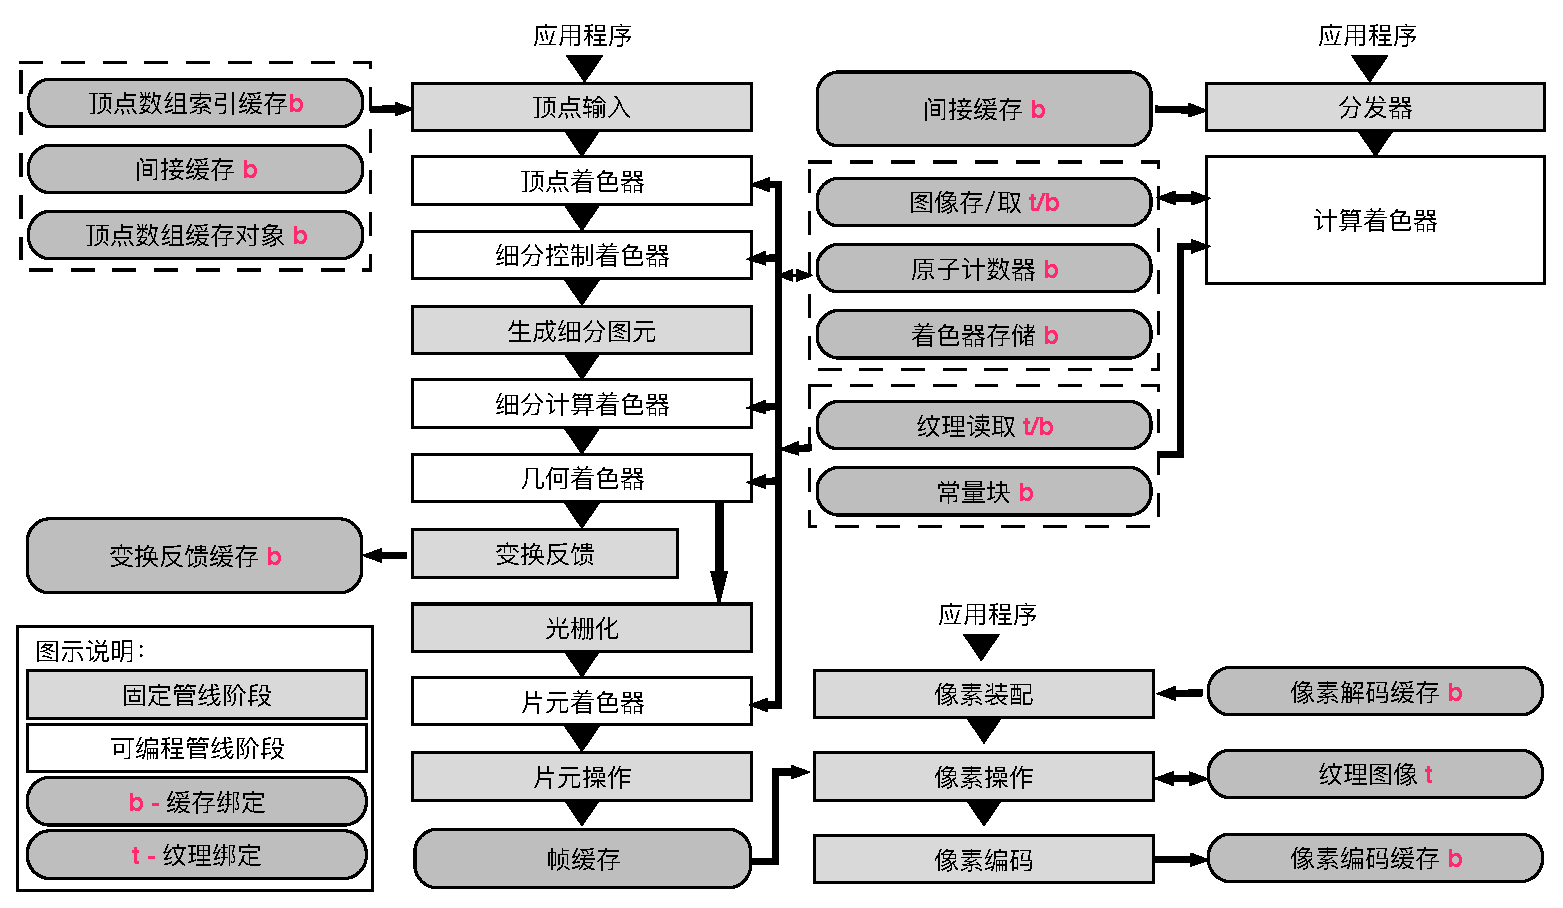
\includegraphics[width=\thewidth]{figures/api/pipeline}
	\caption{OpenGL图形接口执行中的数据流,该图完整展现了OpenGL图形接口中的两种渲染管线:光栅化渲染管线以及计算着色器管线,以及这些计算环节中的数据对象的使用。}
	\label{f:api-pipeline}
\end{fullwidth}
\end{figure}

当我们设置完各种OpenGL对象的状态,以及绑定这些对象到着色器中的属性索引,并将这些对象(包括着色器对象)上传到GPU之后,OpenGL执行环境便开始执行各种管线。对于OpenGL管线,我们首先应该明白的是它不仅仅包括传统经典的光栅化管线,它还可以是纯粹在GPU执行并行计算的计算管线,如图\ref{f:api-pipeline}右上角的计算着色器所示,这种计算着色器可以用来做一些非渲染的计算,如物理模拟,并且计算着色器可以直接读取之前光栅化管线存储在OpenGL对象中的计算结果。此外,我们还可以将渲染管线中对顶点的处理结果存储在变换反馈缓存中,并且终止片元着色器的执行,这可以用来使用GPU进行一些变换或者细分操作,并将这些操作结果读回到宿主程序或者供后续的管线作为顶点数据使用。

在这些基础之上,理解经典的光栅化渲染管线就是再简单不过的事情了。经典渲染管线的目标是把一个虚拟摄像机可视范围内的场景渲染到一个帧缓存对象中,这个帧缓存对象其实是一个容器对象,它包含多个矩形区域的颜色,深度及模板缓存,这些矩形的尺寸对应于摄像机的分辨率。在这个过程中,应用程序输入的是场景中物体的各个顶点相关的数据,例如顶点坐标,每个顶点会在顶点着色器阶段被执行一次顶点着色器计算,在这个阶段可以对每个顶点的属性进行一些处理,例如坐标变换,我们也可以做一些顶点级别的光照计算,顶点着色器输出的结果可以被光栅化器按图元类型进行插值计算。顶点着色器最重要和必须的内容,是将顶点的坐标由世界坐标系变换到由摄像机远近平面及范围(及视锥体)所在的坐标系下,这样后续的管线阶段将可以直接把这些坐标值投影到摄像机对应的屏幕范围,摄像机定义的视锥体可以构造这样一个变换矩阵。

顶点处理的下一个阶段可以对图元进行细分,这通过细分控制着色器和细分计算着色器共同来实现。渲染管线的图元细分可以使得应用程序可以使用更粗粒度的模型顶点表述,减轻CPU和GPU中顶点数据的内存占用以及复杂的顶点数据带来的计算开支,例如坐标变换;图形细分也可以使得渲染管线能够根据分辨率来选择细分的级别,通过减少或增加较远或较近物体的图元数量,来达到更好的渲染性能需求。同时通过后面的变换反馈阶段,渲染管线还可以直接将细分的结果返回到宿主程序,这可以用来加快一些建模工具的实时操作。

几何着色器对每个图元执行一次或多次计算,并输出零个或多个图元。几何着色器的功能使它看起来也可以实现图元细分的功能,然而这不是它的初衷。几何着色器可以对同一个图元执行多次计算用来实现如层级渲染的功能,它也可以用来实现多个输出流来记录不同的顶点数据到不同的变换反馈缓存中。

在顶点处理阶段结束到光栅化阶段之前,我们可以选择终止渲染管线的继续执行,此时可以将经过顶点处理阶段处理过后的顶点信息写入到变换反馈缓存,并将这些数据读回到宿主程序或者用于后续的渲染管线作为输入数据。

之后光栅化阶段对每个图元进行插值,以计算出组成一个图元的所有片元,然后每个片元被后续执行一次片元着色器计算。片元着色器是大部分渲染器实现复杂光照计算的地方,它需要计算出每个片元的颜色值(包含RGBA通道)。随后每个片元再经过片元操作阶段以决定当前片元最终是否被保留,这些片元操作包括深度测试,模板测试,混合计算等。最后,所有通过测试的片元被写入到帧缓存中,供操作系统显示到屏幕上,或者作为后处理的数据进行后续的计算。对于写入到帧缓存中的数据(如颜色,深度,模板值),它们还可以被读回到宿主程序。

在对渲染管线有一个整体的认识之后,本章后面的内容将更详细地描述各个部分的内容。





\section{OpenGL对象}\label{sec:api-opengl-object}
前面我们已经说明,由于CPU和GPU之间隔离的内存和指令执行环境,使得宿主程序并不能直接地和渲染管线进行交互,它们之间只能通过PCI-e或者DMA进行数据传输。这种隔离带来编程结构上的巨大改变,这是学习图形接口或者使用GPU进行并行编程的首要难点之一,它比多核CPU内的并行程序要复杂许多。

GPU编程模型相较于CPU程序最大的区别在于内存对象的使用。首先,由于宿主程序无法拥有GPU内存对象的指针,因此它也需要另外的机制来修改GPU中的内存对象;另一方面,在传统的串行程序中,应用程序通常直接拥有内存对象的地址,因为这些内存对象通常由应用程序直接分配,即内存对象的分配和使用是在同一个环境。然而在GPU并行编程中,内存对象通常并不由这些内核函数(在GPU并行编程中)或着色器(在渲染管线中)直接分配(当然仅供线程内部使用的本地变量除外),因为并行程序在执行的时候会有多个(甚至上千个)实例,所以这些实例只能分配本实例内使用的本地变量,对于全局的变量,它只能由调度这些实例的“宿主”程序进行分配,这就需要一种机制将外部程序分配的全局变量绑定到内核函数中的变量上去。针对上述的两个问题,OpenGL使用两种机制来使用对象。后一种绑定到索引目标的内容将在第\ref{sec:api-buffer-object}节讨论,本节我们讨论前一种机制。

由于宿主程序无法拥有OpenGL对象的指针,所以OpenGL使用一个状态列表来管理OpenGL对象,每个对象都拥有自己的状态列表,不同类型的对象拥有各自不同的状态列表,这些对象状态最终作为整个OpenGL状态的一部分被提交到GPU供着色器或其他固定管线阶段使用。

那么宿主程序怎么设置或者修改这些状态呢?在OpenGL中,所有的对象都是通过以下签名的方法来创建:

\begin{lstlisting}[language=C++]
void glGen*(GLsizei n​, GLuint *objects​);
\end{lstlisting}

该方法为n个OpenGL对象创建n个名称,这些名称存储在objects数组中,每个名称是一个整数,它表示OpenGL服务端一个对象的引用,其中0通常被系统保留。这里*被各种不同的对象类型名称替代,OpenGL中的对象被划分为多种类型,比如Buffer,FrameBuffer,Texture,VertexArray等对象类型,每种类型拥有独立的对象名称,即是说不同类型的对象可能拥有相同的整数名称,因此这些对象在使用的时候必须要指明类型,参见后面的内容。
	

\begin{table}
\begin{fullwidth}
\caption{OpenGL缓存(Buffer)对象的状态列表以及默认值,其中B表示Boolean类型,BMU表示基本的处理器单元,E表示枚举值,$Z^{+}$表示非负整型或枚举值,Y表示指针,S表示终止字符串,$n\times type$表示n个type的复制。}
\label{t:api-buffer-state}
\centering
\begin{tabular}{>{\scriptsize}p{0.29\thewidth}|>{\small}P{0.08\thewidth}|>{\small}P{0.21\thewidth}|>{\scriptsize}P{0.13\thewidth}|>{\small}p{0.25\thewidth}}
\hline 
   状态名称&类型&查询命令&默认值&描述  \\
    \hline  
  -& $n\times BMU$ & GetBufferSubData&-&缓存数据\\
  BUFFER\_SIZE& $n\times Z^{+}$ & GetBufferParameteri64v&0&缓存数据尺寸\\
  BUFFER\_USAGE& $n\times E$ & GetBufferParameteriv&STATIC\_DRAW&缓存使用模式\\
  BUFFER\_ACCESS& $n\times E$ & GetBufferParameteriv&READ\_WRITE&缓存存取标识\\
  BUFFER\_ACCESS\_FLAGS& $n\times Z^{+}$ & GetBufferParameteriv&0&扩展的缓存存取标识\\
  BUFFER\_IMMUTABLE\_STORAGE& $B$ & GetBufferParameteriv&FALSE&如果缓存数据存储可以改变则为TRUE,否则为FALSE\\
  BUFFER\_STORAGE\_FLAGS& $Z^{+}$ & GetBufferParameteriv&0&缓存对象存储标识\\
  BUFFER\_MAPPED& $n\times B$ & GetBufferParameteriv&FALSE&缓存映射标识\\
  BUFFER\_MAP\_POINTER& $n\times Y$ & GetBufferPointerv&NULL&映射的缓存指针\\
  BUFFER\_MAP\_OFFSET& $n\times Z^{+}$ & GetBufferParameteri64v&0&映射缓存范围的起点\\
  BUFFER\_MAP\_LENGTH& $n\times Z^{+}$ & GetBufferParameteri64v&0&映射缓存范围的尺寸\\
  -& $S$ & GetObjectLabel&empty&调试标签\\

 \hline 
\end{tabular}
\end{fullwidth}
\end{table}

那么接下来的问题就是我们怎样修改一个对象的状态值呢?在OpenGL中, 为了修改一个对象的状态值,我们首先需要绑定它们到OpenGL上下文中,这通过如下的OpenGL命令实现:

\begin{lstlisting}[language=C++]
void glBind*(GLenum target​, GLuint object​);
\end{lstlisting}

同样,*表示对象类型,object为要绑定的对象的名称,即是前面glBind*命名分配的名称。其中target参数指示该对象的用途,也可以说它是OpenGL对象类型的进一步划分,同一类型的OpenGL对象拥有类似的使用方法,但是它们在OpenGL中的用途甚至存储结构可能是不一样的。OpenGL使用target来区分不同用途的对象,如表\ref{t:api-buffer-target}所示为OpenGL缓存(Buffer)对象所对应的各种目标名称,读者可以在\cite{b:OpenGL4.5CoreProfile}找到所有其他类型对象所对应的目标名称。

当绑定一个OpenGL对象到一个目标之后,如果该对象之前还没有被绑定过,OpenGL接口即在当前的上下文中为该对象创建一个状态列表\footnote{为什么要在第一次绑定到目标而不是在创建对象名称之后为其创建状态列表,也是因为每个对象的状态列表是与其使用用途相对应的,同一类型(type)的对象可以有多种不同的用途(target),所以具有不同的状态列表。},并使用其类型对应的默认值填充这些状态值\footnote{所以,一个新被创建名称的对象可以被绑定到不同的目标用途上,但是首次绑定决定了该对象的存储位置及布局等,一旦这些信息确定则不能再修改该对象的用途目标。},例如表\ref{t:api-buffer-state}即为一个缓存对象的状态列表及默认值,关于更多OpenGL对象状态的内容可以参考\cite{b:OpenGL4.5CoreProfile}第23章的内容。

当绑定一个OpenGL对象到一个目标之后,后续所有对该目标进行修改的命令均会修改该绑定对象的状态。为什么OpenGL需要用这种方式来修改对象呢?这是因为大部分OpenGL命令的调用都不是立即发送到GPU执行的,它们被保存为一个命令列表,这些前置命令相当于对一个渲染管线的各种设置,这些设置包括对固定管线的控制或者着色器会使用的数据(如纹理和顶点数组),当所有设置完毕之后,我们才通过Draw相关的函数通知GPU执行渲染管线,此时才会将所有这些设置发送到GPU开始执行(包括上传所有OpenGL对象的数据到GPU)。我们可以理解为GPU帮我们执行的是一个叫做“渲染管线”的应用程序,而不是那些OpenGL命令,这些命令只不过是为了执行“渲染管线”这个应用程序所做的配置,相应地我们可以理解OpenGL的状态列表为一个配置表。

我们可以随时查询各个对象的当前状态,根据对象类型的不同,每种类型的对象拥有一套不同的命令来查询其对应的状态,这些命令均可以在\cite{b:OpenGL4.5CoreProfile}中查询到,由于OpenGL上下文的状态在客户端也能读取到,所以这些命令可以立即返回。例如对于缓存对象,它的状态查询命令对应于表\ref{t:api-buffer-state}中的“查询命令”一列的命令名称,例如:

\begin{lstlisting}[language=C++]
void GetBufferParameteriv( enum target, enum pname, int *data );
void GetBufferParameteri64v( enum target, enum pname, int64 *data );
\end{lstlisting}

其中target对应对象的目标名称,pname是每个对象类型拥有的状态名称,它是一个枚举值,而data则包含其查询到的状态数据(根据状态的类型可能是不同类型的数据)。

\begin{table}
\caption{OpenGL缓存类型对象对应的各种不同用途的target名称列表,它们指明这些对象被用于不同的用途。}
\label{t:api-buffer-target}
\centering
\begin{tabular}{>{\small}p{0.56\textwidth}|>{\small}p{0.4\textwidth}}
\hline 
   目标名称 & 用~~途  \\
    \hline  
  ARRAY\_BUFFER                &顶点属性\\
  ATOMIC\_COUNTER\_BUFFER      &高性能原子计数器存储\\
  COPY\_READ\_BUFFER           &缓存复制源\\
  COPY\_WRITE\_BUFFER          &缓存复制目标\\
  DISPATCH\_INDIRECT\_BUFFER   &间接计算着色器分发命令\\
  DRAW\_INDIRECT\_BUFFER       &间接绘制命令参数\\
  ELEMENT\_ARRAY\_BUFFER       &顶点数组索引\\
  PIXEL\_PACK\_BUFFER          &像素读取目标(读回CPU端)\\
  PIXEL\_UNPACK\_BUFFER        &纹理数据目标\\
  QUERY\_BUFFER                &查询结果缓存\\
  SHADER\_STORAGE\_BUFFER      &着色器的读写存储\\
  TEXTURE\_BUFFER              &纹理数据缓存\\
  TRANSFORM\_FEEDBACK\_BUFFER  &变换反馈缓存\\
  UNIFORM\_BUFFER              &着色器的常量块存储\\

 \hline 
\end{tabular}
\end{table}

由于OpenGL通过这种绑定的机制来修改OpenGL对象(的状态),所以当我们修改完一个对象之后,应该立即对该对象进行解绑,以防止后面的命令可能对该对象进行超出预期的修改,否则我们应该始终注意我们所修改的状态属于哪个对象。OpenGL并没有诸如glUnbind之类的命令用来解绑,我们只能通过绑定其他对象到该目标来解除当前对象的绑定,如果我们不再需要对任何对象进行修改,则可以绑定到每种目标对应的默认对象,即名称为0的对象。

当我们不再使用一个对象的时候,使用以下签名的命令删除它:

\begin{lstlisting}[language=C++]
void glDelete*(GLsizei n​, const GLuint *objects​);
\end{lstlisting}

它工作的方式和glGen*类似,只不过这里是删除而不是创建对象。在该命令中,objects参数中任何不合法的对象或者名称为0的对象将会被忽略。当一个对象被删除后,它的名称不再合法,如果该对象已经被绑定到OpenGL当前上下文中,则该对象会被解除绑定。

本节最后我们要讨论的是OpenGL对象的分类,每个OpenGL对象都是具有一定类型的,并且每种类型都分别实现OpenGL某些方面的功能,我们必须分配相应类型的对象来实现特定的功能。除了按用途分类,所有这些对象还可以按是否是容器对象进行划分,表\ref{t:api-object-types}列出了所有的OpenGL的类型划分。

\begin{table}
\caption{OpenGL中的对象类型。}
\label{t:api-object-types}
\centering
\begin{tabular}{>{\small}p{0.5\textwidth}|>{\small}p{0.3\textwidth}|>{\small}p{0.17\textwidth}}
\hline 
   标识符 & 对象类型 & 是否容器  \\
    \hline  
  GL\_BUFFER              &缓存对象 &否\\
  GL\_SHADER              &着色器对象 &否\\
  GL\_PROGRAM             &着色程序对象 &否\\
  GL\_VERTEX\_ARRAY       &顶点数组对象 &是\\
  GL\_QUERY               &查询对象 &否\\
  GL\_PROGRAM\_PIPELINE   &程序管线对象 &是\\
  GL\_TRANSFORM\_FEEDBACK &变换反馈对象 &是\\
  GL\_SAMPLER             &采样器对象 &否\\
  GL\_TEXTURE             &纹理对象 &否\\
  GL\_RENDERBUFFER        &渲染缓存对象 &否\\
  GL\_FRAMEBUFFER         &帧缓存对象 &是\\

 \hline 
\end{tabular}
\end{table}

综合本节的知识,我们可以看出一个对象有类型和用途两种属性,其中类型基本上定义一个对象在接口层面的用法,比如所有缓存对象的用法都是一致的,所有对象类型如表\ref{t:api-object-types}所示;另一方面,一个对象在OpenGL具体被用来做什么,它还需要被绑定到一个用途对应的绑定目标上,例如表\ref{t:api-buffer-target}列出了一个缓存类型的对象可以被绑定的绑定目标。

本节讨论了所有OpenGL对象通用的一些知识,在接下来的几节我们将单独讲述几种比较重要的OpenGL对象,它们的用途以及其他一些特征。





\section{缓存对象}\label{sec:api-buffer-object}
缓存对象(Buffer objects)\index{缓存对象buffer object}\index[en]{buffer object缓存对象}是GPU中一块具有任意尺寸的,无格式的线性内存区域,它是一个字节(byte)数组,可以用来存储顶点数组,从图像或者帧缓存获取的像素数据,或者其他数据,缓存对象在OpenGL中具有广泛的用途,它可以被绑定到多种目标上,见表\ref{t:api-buffer-target}所示。

缓存对象是OpenGL中最重要的对象类型之一,也是使用最复杂的对象类型,因为它无格式要求,因此它几乎可以用来存储OpenGL使用的大部分数据类型(纹理除外);然而也因为它在分配的时候无格式要求的灵活性,使得它在使用的时候却变更复杂,使用者可能需要去区分一个缓存对象中的哪一段数据表示什么样的信息。为了避免在(着色器或OpenGL管线中)使用缓存对象时数据的解析工作,使用缓存对象大部分的复杂性在于需要通过另外一层绑定操作来将告知缓存对象中的各个部分表示什么样的数据,例如当一个缓存用来存储常量数据时,它可以将多个常量以常量块的形式存储在一个缓存对象中。

本节讨论缓存对象除与顶点数组相关以外的所有知识,顶点数组缓存将在第\ref{sec:api-vertex-phase}节顶点处理相关内容中讨论。




\subsection{缓存对象的存储分配}\label{sec:api-buffer-storage}
在定义一个缓存对象的数据存储(Data stores)\index{数据存储data stores}\index[en]{data stores数据存储}之前\footnote{注意,前面的glGen*相关的命令仅仅是为对象分配一个名称,真正的对象创建工作涉及该对象的数据配置,用途等信息的指定。},必须首先绑定到对应用途的目标,缓存对象使用如下的绑定命令:

\begin{lstlisting}[language=C++]
void glBindBuffer​(enum target, uint bufferName);
\end{lstlisting}

其中,bufferName为缓存对象的名称,target为表\ref{t:api-buffer-target}中的目标名称之一,缓存对象作为任何一种用途的数据存储分配的方式都是一致的,所以本小节讨论的内容独立于任何目标名称。同其他OpenGL对象一样,如果该对象第一次被绑定,OpenGL会为其分配该目标对应的状态列表并赋予这些状态默认值,本节讨论的缓存对象数据存储的分配实际上也是缓存对象状态的一部分,参见表\ref{t:api-buffer-state}第一行的数据缓存。

缓存对象在上传数据或被使用之前必须首先为其分配内存,有两种方法可以为缓存对象分配存储:可改变的存储和不可改变的存储。但是不要被这里的名称欺骗,这里的可改变性只是宿主程序与OpenGL的一种约定,它们实际的存储方式是一样的。



\subsubsection{不可改变的存储}
对于不可改变的存储(Immutable storage)\index{不可改变的存储mmmutable storage}\index[en]{mmmutable storage不可改变的存储},它说明宿主程序声明该对象的这块内存一旦分配之后就是固定不变的(例如不可修改大小),但是它的部分或全部内容是可以改变的,这有点类似于C++中常数指针的概念,即这个指针是不可改变的,但是该指针指向的内容是可以改变(以及删除)的,例如:

\begin{lstlisting}[language=C++]
char * const pData = new char[500];     //常数指针
std::fill(pData, pData+500, 0);         //修改全部数据,合法
std::strcpy(pData, "A String Literal"); //修改部分数据,合法
delete []pData;                         //删除对象,合法
pData = new char[700];                  //重新分配内存,不合法
\end{lstlisting}

要对缓存对象分配不可改变的存储,使用以下命令:

\begin{lstlisting}[language=C++]
void glBufferStorage​(GLenum target​, GLsizeiptr size​, const GLvoid * data​, GLbitfield flags​);
\end{lstlisting}

其中,target为使用目标,size表示我们想为缓存对象分配多少字节,data表示指向一个具有size长度的字节数组的指针,OpenGL会在初始化阶段复制data中的数据到GPU,如果data为NULL,则缓存对象的初始数据是未定义的。flags是一个位域(bit field)\index{位域bit field}\index[en]{bit field位域},它用来设定一个宿主程序和OpenGL之间的约定,其描述宿主程序会怎样获取或修改缓存对象的数据。但是,flags的值只会限制客户端对数据存储的修改操作,服务端(server-side)的操作则是始终可用的,所以不管flags的设置是什么,以下操作始终合法:

\begin{itemize}
	\item 在渲染管线内的任何阶段均可以对缓存对象执行写操作,这包括变换反馈,图像加载/存储,原子计数器以及着色器存储缓存对象。
	\item 清除缓存对象的操作,因为该操作只涉及少数字节数据的传输,所以它不被认为是“客户端”修改操作。
	\item 缓存对象之间的复制,因为这始终发生在服务端。
	\item 使缓存对象失效的操作,同清除操作一样,它仅涉及少数数据的传输,所以仍然被认为是“服务端”的操作。
	\item 使用glGetBufferSubData读回缓存对象部分数据到到CPU始终合法。
\end{itemize}

flags位平面的值是如下列表中的值按位或(OR)的结果:

\begin{itemize}
	\item GL\_DYNAMIC\_STORAGE\_BIT:仅当此位被设置时,缓存对象数据存储的数据可以通过BufferSubData命令进行更新,当然缓存对象始终可以被服务端的调用(如ClearBufferSubData和CopyBufferSubData命令)修改。
	\item GL\_MAP\_READ\_BIT:缓存对象的数据存储可以被客户端读映射,映射返回给客户端的指针仅可用于读操作。
	\item GL\_MAP\_WRITE\_BIT:缓存对象的数据存储可以被客户端写映射,映射返回给客户端的指针仅可用于写操作。 
	\item GL\_PERSISTENT\_BIT:允许缓存对象在被映射的时候被使用,如果此位没有设置,则当缓存对象被映射之后的任何操作都会导致错误,当设置此位的时候也必须同时设置其他任意一个与映射相关的位。 
	\item GL\_COHERENT\_BIT:在缓存对象的映射期间,客户端的获取与服务端的使用是连贯一致的。
	\item GL\_CLIENT\_STORAGE\_BIT:建议OpenGL接口实现将数据存储在客户端。
\end{itemize}




\subsubsection{可改变的存储}
为了创建可改变的缓存对象数据存储,使用以下命令:

\begin{lstlisting}[language=C++]
void glBufferData​(enum target, sizeiptr size, const void *data, enum usage);
\end{lstlisting}

前面三个参数都和glBufferStorage是一致的,如果data为NULL,则缓存对象的初始数据是未定义的。由于缓存对象可以以多种方式(或用途)被使用,所以usage参数用来给OpenGL实现一种提示,使其能够以更灵活,高性能的方式存储各种特定用途的缓存对象。

usage用来描述该缓存对象将被怎样使用,它由两个独立的部分组成:即缓存对象将被怎样读和写,以及缓存对象被修改的频率。根据缓存对象将会被怎样读取或写入可以将这些用途分为三类:

\begin{itemize}
	\item DRAW: 宿主程序会向缓存对象写入数据,但是宿主程序不会对其数据进行读取,这些数据仅被OpenGL访问。
	\item READ: 宿主程序不会向其写入数据,但是会读取其数据到CPU,这种缓存数据通常由OpenGL渲染管线产生,例如渲染到一个缓存纹理,写入到变换反馈缓存等。
	\item COPY: 宿主程序不会对缓存对象有任何读取或写入的操作,这种数据通常在OpenGL渲染管线中产生,然后被其他的阶段消费,例如前一帧写入变换反馈缓存的数据作为后一帧的顶点输入。
\end{itemize}

对缓存对象数据的修改主要包括两个方面,其一是宿主程序显式的上传二进制数据到GPU(这包括相应的GL命令可能会修改缓存对象的大小),另一方面是OpenGL的渲染管线(例如着色器内)可能会修改缓存对象的数据。根据缓存对象被修改的频率,可以将这种频率分为三类\footnote{注意,这里的修改频率主要是针对宿主程序的一种约定,因为OpenGL管线内部是始终可以对缓存对象进行修改的。}:

\begin{itemize}
	\item STATIC: 宿主程序只设置缓存对象数据一次,这通常用来设置更新频率非常低的缓存对象。
	\item DYNAMIC: 宿主程序偶尔会修改缓存对象数据,它通常用来设置经常有部分数据被更新的缓存对象。
	\item STREAM: 缓存对象数据几乎在每次使用后都会被宿主程序修改。
\end{itemize}

STREAM, STATIC及DYNAMIC可以和READ, DRAW及COPY任意组合,例如STREAM\_COPY表示OpenGL渲染管线的某些处理会在每次使用完缓存对象的数据之后重新更新缓存对象的数据,并且该缓存对象不会被宿主程序使用glBufferSubData​或类似的命令修改;而STATIC\_READ意味着缓存对象的数据来自OpenGL端的操作,但是只会读取数据一次。 




\subsection{缓存对象数据的修改}
在上一节中我们讨论了缓存对象的创建以及数据初始化,然而更多时候我们需要在后续的使用中不断对数据的部分或全部进行修改。虽然glBufferData(除了被用于初始化可改变的缓存对象)也可以被用于修改缓存对象数据,然而它的原理是对整个缓存对象的存储进行重新分配,所以如果我们只希望更新缓存对象的一部分数据,则这显然是不合适的。

本节我们将讨论一些针对各种情况对缓存对象的一些修改操作,这包括部分更新,映射,清除,复制,使失效等操作。首先,我们可以使用以下命令对缓存对象的部分数据进行更新:

\begin{lstlisting}[language=C++]
void glBufferSubData​(enum target, intptr offset, sizeiptr size, const void *data)
\end{lstlisting}

其中,offset表示一个对缓存对象开始更新的整型位置,size则是更新的范围,也即是将从data对象中复制数据的范围,这里data对象不能为空。

虽然glBufferSubData能够用来方便的更新缓存对象的部分或全部内容,但是它会导致OpenGL进行一次数据的拷贝操作,这会带有一定的资源浪费。例如,宿主程序中可能有一种算法可以用来产生缓存对象需要的数据(例如从文件中读取的数据),但是我们首先得在CPU内存中为这些数据分配一个临时的内存区域用来存储它,然后将这个数据的指针作为data传输给glBufferSubData。使用glGetBufferSubData读回数据也会遇到类似的问题。

然而,如果能够得到一个缓存对象的“指针”,我们就可以直接将算法产生的数据赋值给这个指针,而不需要一个专门的临时内存区域用来存储整个数据对象。在OpenGL中,我们可以通过如下命令实现一种称为映射的方式来得到一个缓存对象的指针:

\begin{lstlisting}[language=C++]
void *glMapBufferRange​(GLenum target​, GLintptr offset​, GLsizeiptr length​, GLbitfield access​);
\end{lstlisting}

该命令将当前绑定到target的缓存对象的指定数据范围的数据区域映射到客户端的地址空间中,它返回的是一个指向缓存对象数据的指针的形式,但是它指向的并不一定是实际图形处理器用到的内存,offset和length用来指明缓存对象映射的范围,access参数指定了应用程序对于映射后的内存区域的使用方式,它必须是表\ref{t:api-glMapBufferRange-access}中列出的标识符之一。

\begin{table}
\caption{glMapBufferRange的访问模式。}
\label{t:api-glMapBufferRange-access}
\centering
\begin{tabular}{>{\small}p{0.27\textwidth}|>{\small}p{0.7\textwidth}}
\hline 
   标识符 & 解释   \\
    \hline  
  GL\_READ\_ONLY    &应用程序仅对OpenGL映射的内存区域执行读操作 \\
  GL\_WRITE\_ONLY   &应用程序仅对OpenGL映射的内存区域执行写操作 \\
  GL\_READ\_WRITE   &应用程序对OpenGL映射的内存区域可能执行读或写操作 \\

 \hline 
\end{tabular}
\end{table}

当一个缓存对象被映射之后,便可以随时解除该缓存对象的绑定,但是除非使用GL\_MAP\_PERSISTENT\_BIT设置创建的可改变的缓存对象(第\ref{sec:api-buffer-storage}节),否则我们不能调用任何命令导致OpenGL对缓存对象进行读写操作。

当我们使用完了缓存对象映射指针之后,必须使用以下命令解除映射指针以使缓存对象变得重新可用:

\begin{lstlisting}[language=C++]
GLboolean glUnmapBuffer(GLenum target​);
\end{lstlisting}

当我们解除缓存对象映射指针后,该指针将失效不再可用。

缓存对象的部分或全部数据也可以被清除,通常我们将其填充为一个特定的值,清除操作使用以下命令:

\begin{lstlisting}[language=C++]
void glClearBufferData​(GLenum target​​, GLenum internalformat​, GLenum format​, GLenum type​, const void * data​);
void glClearBufferSubData​(GLenum target​, GLenum internalformat​, GLintptr offset​, GLsizeiptr size​, GLenum format​, GLenum type​, const void * data​);
\end{lstlisting}

其中,glClearBufferData用于清除全部数据,而glClearBufferSubData用于清除部分或全部数据,这些命令都不会对缓存对象的存储进行重新分配,这些命令的工作机制类似于后面会讲述的像素传输操作。internalformat用于定义数据在缓存对象中的格式,format和type用于定义data中数据的格式,这里data不是包含整个缓存对象大小的数据,而仅是一个“像素”的大小,这些方法会重复复制data的数据直至填充满整个缓存对象,更多关于像素传输及其格式的内容,参见后面第\ref{sec:api-textures}节的内容。
 
缓存对象的数据也可以从另一个缓存对象(或同一个缓存对象的不同部分)复制。为了在缓存对象之间进行数据复制,我们首先需要绑定复制源(source)和复制目的地(destination)缓存对象到对应的目标(target),然后使用以下命令用于缓存对象之间的数据复制:

\begin{lstlisting}[language=C++]
void glCopyBufferSubData​(GLenum readtarget​, GLenum writetarget​, GLintptr readoffset​, GLintptr writeoffset​, GLsizeiptr size​);
\end{lstlisting}

readtarget表示复制源缓存对象的目标,writetarget表示复制目的地对象的目标,readoffset,writeoffset以及size则用于定义复制数据的范围及位置,需要注意的是当复制源和复制目的地缓存对象为同一对象时,它们之间的范围不应该重叠,否则将导致错误发生,另外这些范围也不能超出各自缓存对象的范围。

OpenGL提供了一种使缓存对象无效的机制,如果一个缓存对象或者它的部分区域是无效的,这意味着它的数据内容是未定义的,关于OpenGL怎样处理无效的机制取决于OpenGL实现本身。需注意的是,所有对该缓存对象的等待执行的命令仍将正常执行,任何对一个失效缓存对象的读取操作仍将读取到它之前的数据,而任何对该缓存对象的写操作也将正常执行(但是这些写入的数据会被抛弃,因为我们已经丢弃了该缓存对象)。

无效的概念来源于这样一个简单的机制,它使OpenGL简单地对一个缓存对象(或者部分区域)后续的操作重新分配一块新的存储区域,这样在该缓存对象失效之前的命令仍然能够访问到该缓存对象原始的数据,因此通过失效的机制我们可以很方便地对缓存对象设置新的数据,而不需要考虑其他命令对原始数据的读取操作导致的数据同步的需求,这也使其成为一种后面即将讲述的流式更新数据的方法。

有三种方法可以用于使缓存对象无效,对于可改变的缓存对象,可以使用glBufferData​命令并使用相同的尺寸以及使用NULL作为data参数;也可以在映射时使用GL\_MAP\_INVALIDATE\_BUFFER\_BIT和GL\_MAP\_INVALIDATE\_RANGE\_BIT作为glMapBufferRange​的参数使其全部或部分无效;最后可以使用以下命令显示地声明一个对象失效:

\begin{lstlisting}[language=C++]
void glInvalidateBufferData​(GLuint buffer​);
void glInvalidateBufferSubData​(GLuint buffer​, GLintptr offset​, GLsizeiptr length​);
\end{lstlisting}





\subsection{缓存对象的流式更新}
上述的关于对缓存对象数据修改的方法或者命令都是直接针对缓存对象的数据本身,本小节我们要讨论的是一种特殊形式的“更新”方法,或者说它本身对缓存对象的数据更新的方法并不会超出上述的那些内容,但是它的实现机制可以给应用程序带来很大的性能优化。

利用GPU进行并行计算的程序往往涉及比较大的数据集,例如图形渲染管线输入的巨大的顶点数组,再加上数据由CPU内存经PCI-e或DMA传输到GPU内存的带宽和速度的限制,宿主程序的命令调用和GPU的应用执行之间存在很大的延迟。传统的GPU并行程序的执行方式是“上传数据-执行并行计算程序”,这样的执行模型就使得整个数据传输延迟的期间,GPU资源完全被浪费了,CPU也需要等待GPU执行完毕才开始上传新的数据。

为了解决这个问题,我们在第\ref{chp:hardware}章第\ref{sec-rp-latency}节的关于延迟隐藏的内容中讨论了数据的流式更新,如图\ref{f:rp-streaming}所示,即将数据打散成多个小块,使内核函数(渲染管线中的着色器等)的执行与传输同时进行,这样就能大大隐藏数据的传输延迟,提高GPU的利用率。然而第\ref{chp:hardware}章讨论的关于内核函数直接读取CPU内存的方式通常需要特定的硬件支持,所以它们往往存在于一些扩展当中,例如AMD的AMD\_pinned\_memory扩展\footnote{请参见:\url{https://www.opengl.org/registry/specs/AMD/pinned_memory.txt}。}。不过所有流式更新的理念是一致的,本节讨论一些OpenGL标准本身支持的对缓存对象的流式更新方法。

OpenGL缓存对象流式更新的基本机制是一个缓存对象在被OpenGL使用的同时,宿主程序可以向其更新数据,这相当于把一整个数据集拆分成多个子集达到类似完全的流式更新的效果,但是这个拆分粒度不必很小,只需要不带来CPU和GPU的空闲即可。流式工作的方式如下:我们首先向缓存对象更新一部分数据,然后调用渲染管线开始使用这部分数据进行渲染;在OpenGL开始执行的同时,宿主程序开始更新另一块数据,以此类推。这种流式更新的机制遵循“更新/使用”的模型,如果小心处理完全不需要考虑数据和执行同步的问题,并且更新操作发生在同一个缓存对象身上,所以几乎不影响整个渲染的执行。

本节将讨论几种不同的流式更新的实现方案,每种方案都有各自的优缺点。其中所有使用可改变的缓存对象的方案都需要首先将usage参数设置为STREAM。


\paragraph{使用多个缓存对象}
首先最简单的方式就是使用多个缓存对象,OpenGL渲染管线在使用其中一个缓存对象时,宿主程序可以开始修改另一个缓存对象。这种方法最主要的问题是需要使用多个缓存对象,以及因此带来的图形接口调用的复杂性。



\paragraph{缓存对象数据重定义}
缓存对象数据重定义(Buffer re-specification)的解决方案是在每次修改缓存对象的数据之前重新分配缓存对象的内存,这种技术也称作缓存孤立(Orphaning)\index{缓存孤立cache orphaning}\index[en]{cache orphaning缓存孤立},它在OpenGL术语上称为使对象失效,它有点类似于C++中重新给一个指针变量分配内存,这时原来的内存并没有删除,如果有其他变量引用了原来的地址,则其仍然可以使用原来的数据,只不过在C++中当我们不再使用原来的对象时需要手动释放内存,而OpenGL会在使用完后自动删除失效的缓存数据。

在OpenGL中有两种方法可以实现缓存孤立。第一种方法是使用glBufferData命令,并且使用NULL作为data参数以及其他和原来缓存一样的size和usage参数,这样OpenGL会为缓存对象重新分配一块一样大小的内存,之前的内存则变得失效,但是它仍然可以被缓存对象在被修改前的命令调用。由于新数据的分配只是一个未定义的NULL,因此不需要担心同步问题,对于重复使用相同尺寸的缓存对象进行切换,OpenGL实现甚至可以直接使用之前使用完毕的存储空间而完全避免内存的分配,这有点类似于使用多个缓存进行切换,但是却不需要做出额外的修改。

第二种方法是使用glMapBufferRange命令并设置GL\_INVALIDATE\_BUFFER\_BIT位,也可以使用glInvalidateBufferData​命令,这些都是在修改数据前使其缓存对象数据无效,后续的数据修改都会被分配到新的存储空间。

缓存孤立的性能取决于具体的OpenGL实现,使用时需要注意的问题是必须确保在修改后没有OpenGL操作会对之前的缓存对象数据进行访问。




\paragraph{缓存更新}
缓存更新(Buffer update)\index{缓存更新buffer update}\index[en]{buffer update缓存更新},是在调用glMapBufferRange的时候设置GL\_MAP\_UNSYNCHRONIZED\_BIT位,它告诉OpenGL完全不需要考虑同步问题,宿主程序会保证不会在任何之前的OpenGL渲染操作还在使用缓存数据之前更新缓存数据的内容。

虽然OpenGL不处理同步问题,但是宿主程序必须保证数据和执行的同步,例如如果宿主程序直接修改缓存数据的部分数据,而这部分数据还会被之前OpenGL命令访问,则该数据在被访问的时候是未定义的,因为这种方法完全是对同一块数据进行修改(而不是之前的缓存孤立的机制)。

这种方案的基本用法是,宿主程序对同一个缓存对象进行渐进式更新,每次更新一小块(部分)数据,然后调用OpenGL渲染管线使用这块数据,同时开始更新下一块数据,如此重复,每次更新的数据之间是不重叠的,所以不会有同步的问题。然而一旦整个缓存对象的数据被填充完(即缓存对象的最后一块数据被修改后),则需要一种机制来使该过程可以重新开始,这可以通过两种方法来实现:其一是使用前面的缓存孤立方法重新分配一块新的数据并使之前的数据区域失效,另一种方法是使用OpenGL的同步机制。





\subsection{绑定缓存对象到索引目标}\label{sec:api-indexed-target}
在OpenGL中,有些缓存目标的绑定可以存在多个绑定点,即是多个缓存对象可以用来做类似的事情,例如着色器全局变量(Uniform)可以被划分为多个组,每个组表示本章后面即将讨论的一个接口块,每个接口块的数据用一个单独的缓存对象(或者缓存对象的一部分区域)存储。这时,相同的的目标就具有多个绑定点,此时我们不光要将缓存对象绑定在绑定目标上,还需要将其绑定在这个特定的接口块上,OpenGL会为每个接口块分配一个整型的位置,我们称这样的目标为索引目标(Indexed targets)\index{索引目标indexed targets}\index[en]{indexed targets索引目标},它通过以下的命令实现:

\begin{lstlisting}[language=C++]
void BindBufferRange(enum target, uint index, uint buffer, intptr offset, sizeiptr size);
void BindBufferBase(enum target, uint index, uint buffer);
\end{lstlisting}

其中,target必须是ATOMIC\_COUNTER\_BUFFER, SHADER\_STOR-\\AGE\_BUFFER, TRANSFORM\_FEEDBACK\_BUFFER 和 UNIFORM\_BU- FFER之一。这些变量都是可以在着色器中声明的,它们的具体用途将在本章后面讲述。当这些变量被定义在着色器中之后,在着色器的编译和链接阶段将会为每个接口块分配一个索引值,这个索引值就作为index参数的值,而offset和size用来指定缓存对象的哪部分数据被用来绑定到该接口块上。




\section{着色器和着色器程序}
OpenGL渲染管线中的其中一些阶段是可编程的,例如图\ref{f:api-pipeline}中那些白色背景的阶段,这意味着我们可以编写一段程序,然后OpenGL渲染管线在这些阶段可以执行这些程序。这就要求OpenGL提供一种机制将这些可执行程序发送到GPU,并告诉渲染管线分别应该在不同的可编程阶段使用那段程序。

着色器对象和着色器程序对象是一类特殊的OpenGL对象,它们用来封装这些可执行程序(即着色器),以及执行这些着色器需要的各种状态配置。但是这些对象并不遵循一般的OpenGL对象的一些使用方式,如内存分配及绑定等操作。

在OpenGL中,一个着色器对象(Shader object)\index{着色器对象shader object}\index[en]{shader object着色器对象}封装一个特定类型的着色器程序,这段程序由OpenGL着色语言(OpenGL shading language,GLSL)\index{OpenGL着色语言(OpenGL shading language)}\cite{b:TheOpenGLShadingLanguage}编写,这段程序构成一个字符串。同其他应用程序一样,着色器程序也需要经过编译以生成其对应语言的程序片段。在OpenGL中,我们可以通过以下这些命令来完成上述操作:

\begin{lstlisting}[language=C++]
GLuint glCreateShader​(GLenum shaderType​);
void glShaderSource​(GLuint shader​, GLsizei count​, const GLchar **string​, const GLint *length​);
void glCompileShader​(GLuint shader​);	
\end{lstlisting}

这里首先glCreateShader创建一个shaderType类型的着色器对象,shaderType表示OpenGL中的一个可编程阶段,它必须是GL\_VERTEX\_SHADER, GL\_TESS\_CONTROL\_SHADER, GL\_TESS\_EVALUATION\_SHADER, GL\_GEOMETRY\_SHADER, GL\_FRAGMENT\_SHADER和GL\_COMPUTE\_SHADER中的值之一,该命令返回一个整型的着色器名称;glShaderSource用来指定着色器程序的源代码,其中count表示字符串数组string的长度,length表示取字符串数组string中着色器源代码的长度数组,如果length为NULL则表示取整个字符串;最后,glCompileShader用来编译着色器程序。

一个着色器程序就像C++中的各个单独的源文件,要想被OpenGL执行,我们还必须将所有的着色器程序链接起来,形成一个可执行文件。在OpenGL中这个可执行文件由着色器程序对象(Shader program object)\index{着色器程序对象shader program object}\index[en]{shader program object着色器程序对象}封装,一个着色器程序对象通过以下命令创建并将这些着色器对象附属在一起:

\begin{lstlisting}[language=C++]
GLuint glCreateProgram​();
void glAttachShader​(GLuint program​, GLuint shader​);
\end{lstlisting}

当所有合法的着色器被添加到着色器程序之后,就可以对着色器程序进行链接,如果没有错误发生,之后该着色器程序就可以被OpenGL渲染管线使用了,在OpenGL中使用以下命令来使用着色器程序:

\begin{lstlisting}[language=C++]
void glUseProgram(GLuint program​);
\end{lstlisting}

该命令类似于其他OpenGL对象的绑定操作的功能,一般OpenGL使用一个着色器程序对象来提供所有可编程阶段需要的着色器,如上述这样的操作过程;但是OpenGL也提供另外一种方式可以让一个渲染管线的各个阶段的着色器来自于不同的着色器程序对象,这样做的目的是因为根据不同的需求,各种物体或场景的渲染可能需要不同的着色器组合,如果不支持这样做则需要构建大量的具有重复着色器的着色器程序。这通过创建一个着色器程序管线(Program pipeline)\index{着色器程序管线program pipeline}\index[en]{program pipeline着色器程序管线}对象来实现,由于没有太多特殊的知识所以这里不对其进行详细讨论,读者可以阅读\cite{b:OpenGL4.5CoreProfile}等资料进行学习。





\subsection{着色器程序的链接}
OpenGL使用以下命令来链接着色器程序:

\begin{lstlisting}[language=C++]
void glLinkProgram( uint program );
\end{lstlisting}

跟C++程序不同的是,着色器中使用的变量并不包含在着色器程序对象内部,它们通常被独立地存储在缓存对象或其他OpenGL对象中,因此着色器程序的链接必须要告诉每个着色器从内存中的那些对象及位置去获取这些数据;另外,不同阶段的着色器之间是可以传递数据的,例如顶点着色器输出的值被插值后然后作为片元着色器的输入值,这种情况下由于着色器之间并不像C++程序文件那样可以直接引用(每个着色器是完全独立的),所以这也需要链接阶段来确保这些变量之间的正确传递工作,所有这些配置成为着色器程序对象状态的一部分。

着色器对缓存对象数据的访问大体上可以分为三种方式,但是不管访问方式如何,着色器中的每个变量名称在链接的时候都被分配一个整型的位置,在链接完成之后宿主程序需要根据这些位置来绑定相应的OpenGL对象,根据每种变量类型的不同,OpenGL在内部知道怎样读取这些数据的值。

这三种访问方式如下:
\begin{itemize}
	\item \emph{全局变量 }全局变量是可以被所有着色器访问的变量,在OpenGL中相同类型的全局变量通常被存储在一个缓存对象中,每个变量名称都会被分配一个整型的位置,然后每个变量位置被分别绑定到缓存对象的各个区域。关于全局变量的具体内容详见后面第\ref{sec:api-interface-block}节的内容。
	\item \emph{顺序访问 }有些缓存对象的内容会被着色器顺序访问,这些缓存对象的数据本身是某种固定格式的数据(如顶点缓存对象保存的某个顶点属性的值,以及帧缓存上的颜色缓存保存的一个像素的颜色值),每个着色器实例通常按照某种顺序访问这类数组数据的一个元素。这种情况只需要为每个变量分配一个位置,当这个位置被绑定到一个缓存对象之后OpenGL就可以根据相应的格式为每个着色器实例获取到对应数据\footnote{这实际上就是上一章介绍的内存访问合并的概念。}。例如每个顶点着色器读取顶点数组中的一个顶点的数据,每个片元着色器写入一个颜色值到颜色缓存对象。这类变量包括如图\ref{f:api-locations}中的顶点数组缓存,变换反馈缓存以及帧缓存中的颜色缓存。
	\item \emph{乱序访问 }对于纹理对象,着色器必须有随机访问的能力,因此着色器中的每个纹理变量也会被分配一个位置,这个位置用于绑定到某个纹理对象上。但是与顺序访问不同的是,着色器可以随机访问纹理数据\footnote{这也是访问顶点数据和访问纹理对象的方式不同的原因,每个顶点着色器读取的顶点数据是由着色器实例的顺序决定的,实例的顺序实际上就是访问顶点数组的索引值,所以OpenGL直接传给着色器一个顶点属性变量值;而纹理的访问则是需要通过一个方法来实现,因为着色器需要传入纹理坐标来获取纹理值,这个纹理坐标实际上构成纹理数组的一个索引。}。
\end{itemize}

\begin{figure}
\begin{center}
	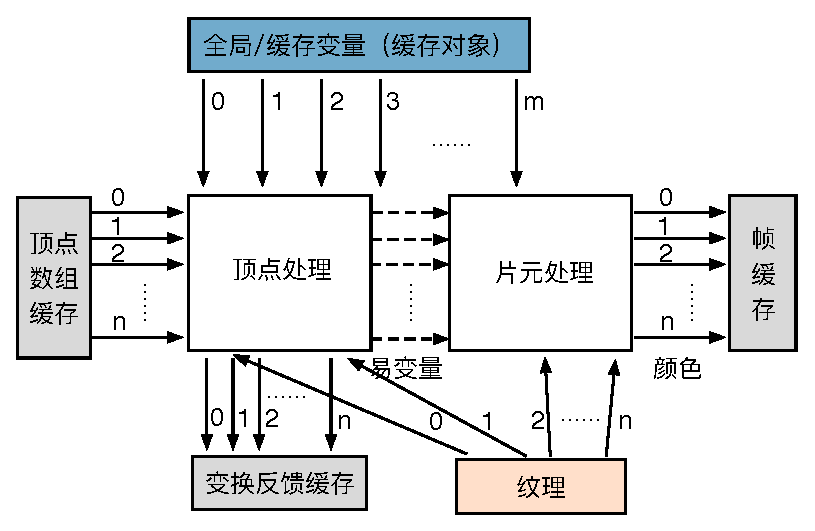
\includegraphics[width=0.75\textwidth]{figures/api/locations}
\end{center}
	\caption{OpenGL渲染管线各个阶段的着色器分散在各自独立的程序中,而这些程序必须从GPU的内存中读取/写入数据,不同阶段的着色器之间也存在联系,所以着色器程序对象的链接必须要处理这些变量和内存之间的关系。}
	\label{f:api-locations}
\end{figure}

上述这些着色器变量的位置在链接之后就会被自动分配,此外,我们还可以在执行链接之前手动给这些变量设定固定的位置,其中对于变换反馈缓存,它必须在链接之前手动设定位置。

总之,在着色器程序链接之后我们就可以查询到这些变量被分配的位置,并且这些位置不能再被更改(除非重新链接),然后宿主程序再将这些变量位置绑定到对应的纹理上面,例如其中一些位置查询的命令如下:

\begin{lstlisting}[language=C++]
GLint glGetAttribLocation​(GLuint program​, const char *name​);
GLint glGetFragDataLocation​(GLuint program​, const char * name​);
GLuint glGetUniformBlockIndex​(GLuint program​​, const char *name​​);
\end{lstlisting}


关于顶点数组缓存,颜色缓存,顶点变换反馈缓存等将在后面对应的渲染管线处理阶段详细讨论,本节我们只讨论跟所有着色器都相关的全局变量。





\subsection{接口块}\label{sec:api-interface-block}
着色器中的变量按照类型分成一些不同的组,每个组是一个接口块(Interface block)\index{接口块interface block}\index[en]{interface block接口块},每种类型可以有多个块,这些类型包括:着色器输入变量(GLSL input),着色器输出变量(GLSL output),全局变量(Uniform)\index{全局变量uniform variables}\index[en]{uniform variables全局变量},以及存储缓存变量(Storage buffer variables)\index{存储缓存变量storage buffer variables}\index[en]{storage buffer variables存储缓存变量}。

不同类型的接口块虽然有各种不同的用途,但是它们的定义是一致的,如下是着色器中一个接口块的定义:

\begin{lstlisting}[language=C++]
storage_qualifier block_name
{
	//在这里定义变量
} instance_name;
\end{lstlisting}

这种结构看起来像一个结构体定义,但实际上它不是一个结构体,因为它直接定义了一些变量(而不是结构体中的对象结构),我们可以直接从这些变量获取数据。storage\_ qualifier可取的值为in,out,uniform和buffer,它们定义接口块的类型,in/out分别表示着色器的输入/输出变量,uniform和buffer表示着色器中的全局变量;block\_name表示接口块的名称,它是宿主程序在查询接口块状态时使用的名称,一个着色器不能同时拥有两个及以上具有相同storage\_qualifier和block\_name的接口块定义。instance\_name是着色器内部用来区分具有相同名称变量的,它是可选的,如果一个接口块具有instance\_name则在着色器内部必须使用它来使用变量,例如如下的接口块定义:

\begin{lstlisting}[language=C++]
uniform MatrixBlock
{
	mat4 projection;
	mat4 modelview;
} matrices;
\end{lstlisting}

为了使用projection变量,必须使用matrices.projection的形式;如果接口块定义不含instance\_name,则直接使用projection引用该变量。block\_name有点类似于命名空间的概念,它用来防止变量名重复导致的歧义,当然任何时候我们都可以使用MatrixBlock.projection的形式来访问变量。

接口块类型in和out用来定义顶点数据,前一阶段着色器输出的易变量等,我们将在本章后面的内容中详细讨论,本节我们主要讨论uniform和buffer类型。




\subsubsection{基于缓存的接口块}
在OpenGL渲染管线中,着色器作为一个内核函数,成千上万的着色器实例在GPU中并行执行。在这些着色器内部,高度结构化的数据(例如顶点数组)被高效地使用如第\ref{chp:hardware}章讨论的全局内存合并这样的技术进行访问,对于只在着色器内部分配和使用的变量,它们被存储在寄存器或者本地存储中,而对于非结构化的可被多个着色器实例共享的数据,在OpenGL中则使用uniform或buffer类型的接口块来存储和使用,这样的接口块称为基于缓存的接口块(Buffer-backed blocks),它包括uniform和buffer两种类型。

在基于缓存的接口块中,整个块中的数据被存储在一个缓存对象(或对象的部分区域)中,并且同一着色器可以包含多个同类型的接口块,为了绑定这些具有相同绑定目标的接口块到多个缓存对象上,OpenGL使用了前面讲述的索引目标的机制,它为每个接口块单独设置一个索引位置,然后将缓存对象同时绑定到绑定目标和索引目标上,参见第\ref{sec:api-indexed-target}节的内容。

uniform和buffer类型接口块中的变量使用的绑定目标分别为GL\_UNIF-\\ORM\_BUFFER和GL\_SHADER\_ STORAGE\_BUFFER,在着色器程序链接之后,每个接口块会被分配一个块索引值,这可以通过以下命令查询:

\begin{lstlisting}[language=C++]
GLuint glGetUniformBlockIndex​(GLuint program​​, const char *name​​);
\end{lstlisting}

这里name是接口块中的block\_name参数。当我们得到这个块索引值后就可以根据第\ref{sec:api-indexed-target}节中讲述的方法将缓存对象绑定到这个索引目标上,为了方便我们这里重新列出该命令:

\begin{lstlisting}[language=C++]
void BindBufferRange(enum target , uint index , uint buffer , intptr offset , sizeiptr size);
void BindBufferBase(enum target, uint index, uint buffer);
\end{lstlisting}

这里index参数即是接口块的索引值。然而第\ref{sec:api-indexed-target}节讲述的绑定方法存在一个问题,当我们选择使用程序管线对象\footnote{回想一个程序管线对象(Program pipeline)可以从多个着色器程序对象中选择不同阶段的着色器来构成一个虚拟的“着色器程序对象”。}而不是着色器程序对象来存储渲染管线需要的着色器时,每个着色器对象分配的接口块的索引值是独立的,所以管线内的接口块索引值可能存在重复。这种情况下我们可以使用以下命令来绑定接口块:

\begin{lstlisting}[language=C++]
void glUniformBlockBinding​(GLuint program​​, GLuint uniformBlockIndex​​, GLuint uniformBlockBinding​​);
void glShaderStorageBlockBinding​(GLuint program​​, GLuint storageBlockIndex​​, GLuint storageBlockBinding​​);
\end{lstlisting}

这里uniformBlockIndex和storageBlockIndex分别是对应program链接后产生的块索引值,uniformBlockBinding和storageBlockBinding的值可以分别通过以下方法调用查询得到:

\begin{lstlisting}[language=C++]
glGetActiveUniformBlockiv( program, uniformBlockIndex, GL_UNIFORM_BLOCK_BINDING, &uniformBlockBinding );
glGetActiveUniformBlockiv( program, storageBlockIndex, GL_SHADER_STORAGE_BINDING, &storageBlockBinding );
\end{lstlisting}

接口块块索引值也可以直接通过着色器内部设置,例如:

\begin{lstlisting}[language=C++]
layout(binding = 3) uniform MatrixBlock
{
	mat4 projection;
	mat4 modelview;
};
\end{lstlisting}

uniform和buffer类型的接口块分别拥有自己独立的块索引值集,uniform块的索引值用于绑定到GL\_UNIFORM\_BUFFER目标上,buffer块的索引值用于绑定到GL\_SHADER\_STORAGE\_BUFFER目标上。块也可以构成数组,它的定义方法如下:

\begin{lstlisting}
layout(binding = 2) uniform MatrixBlock
{
	mat4 projection;
	mat4 modelview;
} matrices[4];
\end{lstlisting}

这会产生4个独立的uniform块,它们的块索引值分别为2,3,4和5。所以它们虽然使用起来像数组,但其实是被分别存储在不同的缓存对象中的。

那接口块内的变量怎样从缓存对象中取得数据呢?在OpenGL中,每个接口块内的每个变量按顺序具有一个索引值,每个变量类型决定了其所占据的长度,这些信息可以用来计算每个变量的数据在缓存对象内的偏移值,所有这些信息都被记录在着色器程序状态数据中,OpenGL就可以知道怎样获取接口块内每个变量的值。

要查询这些信息,首先需要取得每个变量在接口块内的索引值\footnote{注意,这里的变量索引值是接口块内的每个变量的索引值,而不是接口块的索引值,后者用来绑定到缓存对象上,而变量索引值用来获取变量的数据,以及对缓存对象中的相应区域赋值。},这通过以下命令实现:

\begin{lstlisting}[language=C++]
void glGetUniformIndices(GLuint program​, GLsizei uniformCount​, const GLchar **uniformNames​, GLuint *uniformIndices​);
\end{lstlisting}

其中,uniformNames表示要查询的变量的名称数组,uniformCount指示数组中变量名称的数量,这些变量的索引值都存储在uniformIndices数组中。

当得到接口块内一个变量的索引值之后,就可以通过以下命令查询该变量的一些状态信息:

\begin{lstlisting}[language=C++]
void glGetActiveUniformsiv(GLuint program​, GLsizei uniformCount​, const GLuint *uniformIndices​, GLenum pname​, GLint *params​);
\end{lstlisting}

该命令查询索引数组uniformIndices中的uniformCount个索引值表示的变量的状态名称为pname的值,这些值的查询结果存储在数组params中。params的值可以是GL\_UNIFORM\_SIZE和GL\_UNIFORM\_OFFSET,它们分别表示该变量的大小以及变量的数据在缓存对象中的偏移值,这些值可以用来帮助宿主程序向缓存对象填充数据,例如我们可以使用memcpy函数来向缓存对象复制值到对应的区域。该命令还可以查询其他一些状态信息,例如GL\_UNIFORM\_NAME\_LENGTH,GL\_UNIFORM\_BLOCK\_INDEX,GL\_UNIFORM\_ARRAY\_STRIDE,GL\_UNIFORM\_MATRIX\_STRIDE,GL\_UNIFORM\_IS\_ROW\_MAJOR,GL\_UNIFORM\_ATOMIC\_COUNTER\_B- UFFER\_INDEX,相关的内容读者可以阅读\cite{b:OpenGL4.5CoreProfile}。

当然所有这些命令同样可以用在buffer块上,uniform块与buffer块最大的区别在于,着色器存储缓存可以在着色器中读写,通过缓存块写入存储数据的内容也可以被其他着色器请求使用,并且可以读回到应用程序。





\subsection{接口匹配}
渲染管线中不同阶段着色器都具有一些输入和输出值,大多数时候前一个管线阶段输出(out块)的值被后一个相邻阶段的着色器消费(in块),因此在链接\footnote{注意,当使用来自多个着色器程序对象中的不同阶段的着色器执行一个渲染管线时(即使用着色器程序管线对象时),这种匹配工作只能在运行时检测,本章将不会讨论这方面的内容,读者请自行阅读OpenGL文档。}着色器程序的时候,OpenGL还必须做接口匹配(Interface matching)\index{接口匹配interface matching}\index[en]{interface matching接口匹配}工作,不匹配的输入输出接口将导致链接失败。

接口匹配主要涉及两个或多个着色器内部某些接口块的定义保持一致,它包含两方面的匹配:一个是相邻两个阶段的着色器内in/out块之间的匹配,另一个是多个着色器内uniform和buffer块的匹配。

首先,多个阶段的着色器的链接要求所有前一阶段着色器输出的接口块必须被后一阶段的着色器消费,反之,所有后一阶段着色器中的输入值必须匹配前一阶段着色器的输出值(顶点着色器除外)。这个匹配工作是必须的,因为存储这些输入输出值的缓存对象是渲染管线的一些中间产物,它并不需要我们手动去维护(例如分配和绑定)这些缓存对象(最后阶段输出的颜色缓存除外),这样相邻两个着色器对这些中间缓存对象的使用必须遵循一些规则,才能使OpenGL知道怎么去使用这些缓存对象,例如使用匹配的接口块定义则可以让OpenGL知道每个着色器实例的每个接口块对应于缓存对象的哪一段数据,以及每个接口块内部的每个变量的数据来自缓存对象的哪一段范围。

输入输出接口块匹配的规则如下:

\begin{itemize}
	\item 两个块定义的块名称必须相同,注意块名称是可以被宿主程序访问的block\_name,而不是着色器内部充当命名空间功能的instance\_name。
	\item 输出块和输入块的成员变量的定义要完全相同。

\end{itemize}

对于上述第二个规则,这意味着:

\begin{itemize}
	\item 所有变量以相同的顺序定义。
	\item 每个对应变量具有相同的名称。
	\item 每个对应变量具有相同的类型,如果该变量为数组变量,则其长度相等。
	\item 其他一些关于类型标识符的匹配规则请参见\cite{b:OpenGL4.5CoreProfile}。
\end{itemize}

例如以下顶点着色器的输出块:

\begin{lstlisting}
out Lighting 
{
	vec3 normal;
	vec3 bumpCorrd;
};
\end{lstlisting}

匹配片元着色器的输入块:

\begin{lstlisting}
in Lighting 
{
	vec3 normal;
	vec3 bumpCorrd;
};
\end{lstlisting}


此外,对于输入输出块,它们还可以以一种比较松散的方式定义,例如:

\begin{lstlisting}[language=C++]
layout(location = 1) out vec3 three;
\end{lstlisting}

此时,输入输出接口块的匹配除了要求变量名称,数据类型以及数组的长度之外,还必须在绑定位置要保持一致,即如果其中一个包含有着色器内location(块索引)的指定,则输入输出块必须都包含location的指定并且块索引的位置相等,否则它们可以都不包含location的着色器内指定。

对于uniform/buffer块,它们的匹配规则基本和上述规则一致,除了它们的块类型必须一致,即都为uniform块或都为buffer块。

关于接口块的匹配在使用着色器程序管线对象时还涉及其他一些规则,接口块本身也还存在其他一些内容例如可以控制矩阵变量的数据布局方式(行优先还是列优先),由于本书不是专门讲述OpenGL知识的书籍,请读者自行参考OpenGL文档,本章仅讨论OpenGL的一些核心功能尤其是它们之间的一些联系。





\section{纹~~理}\label{sec:api-textures}
缓存对象可以用来存储任意格式的数据,只要OpenGL知道以怎样的方式从缓存对象的存储中去读取这些数据,例如它既可以用来存储结构化的顶点数组数据,也可以在着色器中以buffer块的形式存储完全自由结构的数据。缓存对象的使用通常只需要OpenGL与宿主程序之间建立一种格式协议,这种协议用来给每个变量获取一个地址,在使用的时候,OpenGL就可以直接从这个地址读取缓存对象存储中的数据。因此缓存对象在OpenGL眼里就是一个变量。

纹理(Texture)对象在很多方面不同于缓存对象。首先,纹理对象是高度格式化的,特别地,纹理的格式以颜色为基础,并且它具有维度;其次,不同于缓存对象存储的是一些离散的精确的值,纹理对象的数据表示的是某个作用域下的某个特征值的分布,例如一个2D的纹理可以表示一个物体表面颜色的分布,而一个3D的纹理可以表示一个体积内的介质浓度分布,如果我们能够以一个具有少数变量表示的多项式来表征这些同样的分布,那么一个纹理对象完全可以使用这个公式来代替,因此纹理对象的数据存储的是一个函数。

由于纹理对象以离散的值来存储一个函数,那么纹理对象存储空间里的值对于我们并没有特别的意义(尤其当纹理对原连续函数的采样率小于其在摄像机空间内的分辨率的2倍时),我们需要的是一个函数值,从一个离散的函数中进行采样就必须要对离散函数进行重建以还原原始连续函数,然后得到的值才是有意义的函数值。因此纹理在OpenGL眼里不能仅仅当做一个变量使用,它必须包含一个采样的方法,它还需要一些参数来控制对纹理分布函数的采样。

尽管纹理的数据也可以像缓存对象那样被直接读取和使用,但是把纹理当做一个离散分布函数的概念有助于我们更深刻地理解它的概念。在本章乃至本书我们都会始终以这样的方式来讨论纹理的概念及其相关的应用。

在OpenGL中,纹理是一个包含一个或多个图像\footnote{注意,纹理并不能包含任意数量的图像,图像的数量通常是由纹理类型本身决定的。}(Image)\index{图像image}\index[en]{image图像}的容器对象。纹理有三个属性:纹理类型,纹理尺寸以及图像格式,纹理的类型(如表\ref{t:api-texture-type}所示)定义纹理内的图像如何排列,纹理的尺寸定义纹理中每个图像的尺寸,每个图像是一个1D,2D或3D的像素的数组,图像格式(Image format)\index{图像格式image format}\index[en]{image format图像格式}则定义每个像素的格式,纹理中的像素通常称为纹素(texel)\index{纹素texel}\index[en]{texel纹素}。

\begin{table}
\begin{fullwidth}
\caption{OpenGL中纹理的类型,以及对应的采样器类型,纹理的类型决定纹理内的图像如何排布以及图像的维度等信息}
\label{t:api-texture-type}
\centering
\begin{tabular}{>{\footnotesize}p{0.27\thewidth}|>{\small}p{0.19\thewidth}|>{\small}p{0.52\thewidth}}
\hline 
   目标GL\_TEXTURE\_* & 采样器类型 & 描述 \\
    \hline  
  1D  &sampler1D &所有图像都是1维的,它具有宽度,没有高度和深度\\
  2D  &sampler2D &所有图像都是2维的,它具有宽度和高度,没有深度\\
  3D  &sampler3D &所有图像都是3维的,它具有宽度,高度和深度\\
  RECTANGLE  &samplerRect &只包含一个2维的图像,并且没有mipmap,用于采样的纹理坐标没有被归一化\\
  BUFFER  &samplerBuffer & 只包含一个1维的图像,没有mipmap,纹理的数据存储在一个缓存对象中\\
  CUBE\_MAP &samplerCube& 包含6个2维的图像集合,每个图像具有相同的尺寸,表示一个立方体的6个面\\
  1D\_ARRAY &sampler1DArray& 包含多个1维图像的集合,它的尺寸包括数组的长度\\
  2D\_ARRAY &sampler2DArray& 包含多个2维图像的集合,它的尺寸包括数组的长度\\
  CUBE\_MAP\_ARRAY &sampler1DCubeArray& 包含多个立方体图像的集合,数组的长度*6是纹理尺寸的一部分\\
  2D\_MULTISAMPLE &sampler2DMS& 只包含一个2维的图像,没有Mipmap,但是每个像素包含多个采样点(而不是一个)\\
  2D\_MULTISAMPLE\_ARRAY &sampler2DMSArray&包含多个2维多重采样纹理图像的集合\\

 \hline 
\end{tabular}
\end{fullwidth}
\end{table}




\subsection{纹理的创建}\label{sec:api-texture-create}
纹理对象遵循第\ref{sec:api-opengl-object}节OpenGL对象的创建和管理方式,一个纹理对象通过以下命令创建对象名称:

\begin{lstlisting}[language=C++]
void glGenTextures(GLsizei n, GLuint* textures);
\end{lstlisting}

当纹理的名称被创建后,它还没有维数和类型,只有第一次绑定到目标后才能决定其类型,初始绑定的目标决定了创建的纹理类型,从这时起,纹理将只会被绑定到这个目标上,直到被销毁为止。

纹理的绑定使用如下命令:

\begin{lstlisting}[language=C++]
void glBindTexture(GLenum target, GLuint texture);
\end{lstlisting}

其中,target为表\ref{t:api-texture-type}中的目标类型之一。

在OpenGL着色器中可以使用多个纹理,类似于前面讲述的索引目标,OpenGL为每个纹理分配一个整数的索引,称为纹理单元(Texture unit)\index{纹理单元texture unit}\index[en]{texture unit纹理单元},所以和索引目标一样,每个纹理对象还必须绑定到对应的纹理单元。但是纹理单元的绑定方式则和索引目标不一样,要绑定纹理对象到某个纹理单元,我们需要在glBindTexture命令之前使用以下命令:

\begin{lstlisting}[language=C++]
void glActiveTexture(GLenum texture);
\end{lstlisting}

该命令激活一个纹理单元,然后后续的对纹理的操作都会被关联到这个纹理单元上。在OpenGL着色语言中纹理必须通过一个采样器来对其进行采样\footnote{回想纹理数据是一个分布函数。},所以着色器使用的纹理单元数量通过采样器变量的数量来决定。

在OpenGL着色语言中,采样器变量被定义为一个uniform类型的变量,设想着色器中定义以下两个采样器变量:

\begin{lstlisting}[language=C++]
uniform sampler2D tex1;
uniform sampler2D tex2;
\end{lstlisting}

则在宿主程序中可以通过以下方式来绑定各个纹理到对应的纹理单元:

\begin{lstlisting}[language=C++]
glUseProgram(prog);

GLint tex1_uniform_loc = glGetUniformLocation(prog, "tex1");
glUniform1i(tex1_uniform_loc, 0);
glActiveTexture(GL_TEXTURE0);
glBindTexture(GL_TEXTURE_2D, tex1);
 	
GLint tex2_uniform_loc = glGetUniformLocation(prog, "tex2");
glUniform1i(tex2_uniform_loc, 1);
glActiveTexture(GL_TEXTURE1);
glBindTexture(GL_TEXTURE_2D, tex2);
\end{lstlisting}

不同于索引目标被OpenGL自动分配(当然也可以通过在着色器中使用location手动分配),纹理单元需要手动分配,纹理单元的值是OpenGL定义的一系列枚举值,分别命名为GL\_TEXTURE$i$,其中$i$在0到$k-1$范围,$k$表示纹理单元的最大数目,所以GL\_TEXTURE$i$的值等于GL\_TUXTURE0+$i$。这里的代码首先将纹理的变量通过glUniform1i设置为一个纹理单元的值,然后再将该纹理单元激活以使后面的纹理对象被绑定到该纹理单元上。

在创建一个纹理对象之后,必须为它设置存储和数据。纹理对象的存储也和缓存对象一样具有可改变和不可改变之分,只不过纹理的可改变不光包括存储的位置和大小,还包括纹理的格式和尺寸。

我们先来看不可改变的存储分配,这些命令如下:

\begin{lstlisting}[language=C++]
void glTexStorage1D(GLenum target, GLsizei levels, GLenum internalFormat, GLsizei width);
void glTexStorage2D(GLenum target, GLsizei levels, GLenum internalFormat, GLsizei width, GLsizei height);
void glTexStorage3D(GLenum target, GLsizei levels, GLenum internalFormat, GLsizei width, GLsizei height, GLsizei depth);
\end{lstlisting}

纹理对象的每1维都有相关的决定纹理边界的存储函数的定义,对于数组纹理可以下一个更高维来设置数组的大小,例如用glTexStorage2D为1维数组纹理初始化存储,用glTexStorage3D为2维数组纹理初始化存储。这三个命令为纹理创建固定存储,即纹理的内部格式,大小,类型以及mipmap的级数都不能再改变。当然和不可改变的缓存对象一样,这也只是存储本身不能改变,但是纹理的内容可以被后面会讨论的glTexSubImage2D等命令来改变。

对应的可改变存储的纹理对象的命令如下:

\begin{lstlisting}[language=C++]
void glTexImage1D(GLenum target, GLint level, GLint internalFormat, GLsizei width, GLint border, GLenum format, GLenum type, const void *data);
void glTexImage2D(GLenum target, GLint level, GLint internalFormat, GLsizei width, GLsizei height, GLint border, GLenum format, GLenum type, const void *data);
void glTexImage3D(GLenum target, GLint level, GLint internalFormat, GLsizei width,GLsizei height, GLsizei depth, GLint border, GLenum format, GLenum type, const void *data);
\end{lstlisting}

这里列出的纹理内部格式,大小,mipmap级数以及纹理数据都可以被每次调用这些命令的时候改变。同样,glTexImage*命令的data数据可以来自CPU内存中的一个指针,或者GPU中的一个缓存对象的偏移值,当从缓存对象复制数据时,其缓存必须要被绑定到GL\_PIXEL\_UNPACK\_BUFFER目标上,我们将在下一节讨论这种限制的原因,以及讨论internalformat,format和type这些参数的意义。此外,对于多重采样的纹理还有各自独立的存储创建函数,请读者自行参考OpenGL文档\cite{b:OpenGL4.5CoreProfile}。





\subsection{像素传输}
上一节讲述的glTexImage*以及本节要讨论的其他一些命令涉及像素数据在客户内存和GPU设备内存之间的传输,这称为像素传输(Pixel transfer)\index{像素传输pixel transfer}\index[en]{pixel transfer像素传输}。客户内存的数据通常是未格式化的,我们称之为编码的(packed),所以像素传输由客户内存向设备内存的过程称为像素解码(Pixel unpack)\index{像素解码pixel unpack}\index[en]{pixel unpack像素解码}操作,而由设备内存向客户内存传输的过程称为像素编码(Pixel pack)\index{像素编码pixel pack}\index[en]{pixel pack像素编码}操作。

\begin{myshaded}
	计算机中的数据为什么需要编码和解码?这是因为通常程序需要处理来自外部的数据,也因此可能会写入数据到外部,这个外部可能是网络的另一端,它使用另一种不同的语言来处理这些数据,例如来自网络服务器端被Ruby程序写入的数据被客户端的C++程序使用。当数据在两种不同的系统之间传输时,两种系统之间对数据类型的支持是不一样的,例如宿主C++程序支持GLbyte, GLubyte, GLshort, GLushort等类型,而OpenGL服务端对于纹理对象只支持整型和浮点数两种类型,这种情况下数据的传输就需要编码和解码操作。
	
	编码操作通常接收一个模板字符串,以及该系统支持的数据类型的一些变量的值,然后返回一个标量,例如网页请求时服务端将一些数据拼成一个字符串的格式传输给客户端;解码则相反,它接收一个标量的编码数据,以及同样的模板字符串,它在使用这些数据的系统将这些信息解析出来并使用该系统支持的数据类型表示。
\end{myshaded}

在OpenGL中,像素数据由设备内存传输到客户内存(编码)的命令包括:

\begin{itemize}
	\item glReadPixels: 从当前绑定的帧缓存中读取像素数据到客户端内存。
	\item glGetTexImage: 读取当前绑定的某个纹理对象中某个mipmap级别的所有的数据到客户端内存。
\end{itemize}

反之,像素数据由客户内存传输到设备内存(解码)的命令包括:

\begin{itemize}
	\item glTexImage*: 为一个纹理对象的某个mipmap级别分配可改变的存储空间,该命令也可用直接传输数据,见第\ref{sec:api-texture-create}节的内容。
	\item glTexSubImage*: 将客户内存中的纹理数据写入到一个当前绑定的纹理对象的某个mipmap级别。
\end{itemize}

此外,OpenGL还为压缩纹理提供一些特殊的传输命令,但是正如第\ref{sec:api-compressed-texture}节即将讨论的那样,压缩纹理的传输不涉及任何数据的转换操作,它们只是直接将数据传输到设备内存中,这是因为客户内存中的压缩纹理的数据本身就是按照OpenGL要求的格式存储的。





\subsubsection{像素传输参数}
尽管本章只涉及像素解码操作,但是像素传输的参数是一致的,所以本节一起讨论它们。除了压缩纹理外,所有关于像素传输的操作都涉及4个参数:

\begin{lstlisting}[language=C++]
GLint internalFormat, GLenum format​, GLenum type​, void *data​
\end{lstlisting}

这里data是一个客户内存的指针或者一个缓存对象的偏移值,当进行像素解码操作的时候,该缓存对象的绑定目标必须是GL\_PIXEL\_UNPACK\_BUFFER,当进行像素编码操作的时候,该缓存对象的绑定目标必须是GL\_PIXEL\_PACK\_BUFFER。为了方便,以下我们仅称其为“客户内存”,不管其是客户内存的指针还是缓存对象的偏移。

内部格式(Internal format)\index{内部格式internal format}\index[en]{internal format内部格式}决定了OpenGL在设备内存存储纹理的格式,完整的内部格式由基本格式的标识符,一个或更多大小的标识符和可选的数据类型组成,即GL\_[components][size]\_[type]。基本格式决定了提供的纹理分量,例如以GL\_R开头的格式只有红色分量,以GL\_RG开始的格式有红色和绿色分量,完整的基本格式参见表\ref{t:api-texture-base-internal-format}。

\begin{table}
\caption{内部基本格式像颜色,深度和模板分量的转换}
\label{t:api-texture-base-internal-format}
\centering
\begin{tabular}{>{\small}p{0.3\textwidth}|>{\small}p{0.4\textwidth}|>{\small}p{0.28\textwidth}}
\hline 
   基本格式 & RGBA,深度和模板值 & 内部分量构成 \\
    \hline  
  DEPTH\_COMPONENT  &Depth           &$D$\\
  DEPTH\_STENCIL    &Depth,Stencil  &$D,S$\\
  RED               &R               &$R$\\
  RG                &R, G            &$R, G$\\
  RGB               &R, G, B         &$R, G,B$\\
  RGBA              &R, G, B, A      &$R, G, B, A$\\
  STENCIL\_INDEX    &Stencil         &$S$\\

 \hline 
\end{tabular}
\end{table}

大小标识符决定了用来存储纹理数据的位数,如表\ref{t:api-texture-sized-internal-format}所示,在许多情况下只包括一个大小参数,也可以分别为每个分量指定大小。OpenGL默认以无符号归一化格式存储纹理,当数据以无符号归一化数据存储时,纹素在内存中以整数存储,整数在读进着色器时转化为浮点数,并且用整数对应的可以表示的最大值来除,这将生成传递给着色器的范围在[0.0,1.0]的数据。如果内部格式提供的是\_SNORM(Signed normalized)修饰符,数据是有符号的归一化,在这种情况下,内存中的数据是有符号整数,同样在返回给着色器时,转化为浮点数,生成范围在[-1.0,1.0]的浮点数据。

\newpage
\begin{longtable}{>{\small}p{0.28\textwidth}|>{\small}p{0.15\textwidth}|>{\small}p{0.1\textwidth}|>{\small}p{0.1\textwidth}|>{\small}p{0.1\textwidth}|>{\small}p{0.1\textwidth}|>{\small}p{0.1\textwidth}}
\caption{OpenGL纹理完整的内部格式定义,包括基本格式标识符,大小标识符以及可选的数据类型}
\label{t:api-texture-sized-internal-format}\\

\hline 
   有大小的内部格式 & 基本内部格式 & R分量 & G分量 & B分量 &A分量 & 共享位 \\
    \hline  
  
  R8            & RED & 8   & &  & &\\ \hline
  R8\_SNORM     & RED & s8  & &  & &\\\hline
  R16           & RED & 16  & &  & &\\\hline
  R16\_SNORM    & RED & s16 & &  & &\\\hline
  RG8           & RG  & 8   & 8  & & &\\\hline
  RG8\_SNORM    & RG  & s8  & s8 & & &\\\hline
  RG16          & RG  & 16  & 16 & & &\\\hline
  RG16\_SNORM   & RG  & s16 & s16 & & &\\\hline
  
  R3\_G3\_B2   & RGB & 3 & 3 & 2 & &\\\hline
  RGB4          & RGB & 4 & 4 & 4 & &\\\hline
  RGB5          & RGB & 5 & 5 & 5 & &\\\hline
  RGB565        & RGB & 5 & 6 & 5 & &\\\hline
  RGB8          & RGB & 8 & 8 & 8 & &\\\hline
  RGB8\_SNORM   & RGB & s8 & s8 & s8 & &\\\hline
  RGB10         & RGB & 10 & 10 & 10 & &\\\hline
  RGB12         & RGB & 12 & 12 & 12 & &\\\hline
  RGB16         & RGB & 16 & 16 & 16 & &\\\hline
  RGB16\_SNORM  & RGB & s16 & s16 & s16 & &\\\hline
  
  RGBA2         & RGBA & 2 & 2 & 2 & 2 &\\\hline
  RGBA4         & RGBA & 4 & 4 & 4 & 4 &\\\hline
  RGB5\_A1      & RGBA & 5 & 5 & 5 & 1 &\\\hline
  RGBA8         & RGBA & 8 & 8 & 8 & 8 &\\\hline
  RGBA8\_SNORM  & RGBA & s8 & s8 & s8 & s8 &\\\hline
  RGB10\_A2     & RGBA & 10 & 10 & 10 & 2  &\\\hline
  RGB10\_A2UI   & RGBA & ui10 & ui10 & ui10 & ui2 &\\\hline
  RGBA12        & RGBA & 12 & 12 & 12 & 12 &\\\hline
  RGBA16        & RGBA & 16 & 16 & 16 & 16 &\\\hline
  RGBA16\_SNORM & RGBA & s16 & s16 & s16 & s16 &\\\hline
  
  SRGB8         & RGB  & 8 & 8 & 8 & &\\\hline
  RRGB8\_ALPHA8 & RGBA & 8 & 8 & 8 & 8 &\\\hline
  R16F          & RED  & f16 & & & &\\\hline
  RG16F         & RG   & f16 & f16 & & &\\\hline
  RGB16F        & RGB  & f16 & f16 & f16 & &\\\hline
  RGBA16        & RGBA & f16 & f16 & f16 & f16 &\\\hline
  
  R32F          & RED  & f32 & & & &\\\hline
  RG32F         & RG   & f32 & f32 & & &\\\hline
  RGB32F        & RGB  & f32 & f32 & f32 & &\\\hline
  RGBA32        & RGBA & f32 & f32 & f32 & f32 &\\\hline
  
  R11F\_G11F\_B10F  & RGB & f11 & f11 & f10 & &\\\hline
  RGB9\_E5          & RGB & 9   & 9   & 9 & & 5\\\hline
  
  R8I           & RED & i8 & & & &\\\hline
  R8UI          & RED & ui8 & & & &\\\hline
  R16I          & RED & i16 & & & &\\\hline
  R16UI         & RED & ui16 & & & &\\\hline
  R32I          & RED & i32 & & & &\\\hline
  R32UI         & RED & ui32 & & & &\\\hline
  
  RG8I          & RG & i8 & i8 & & &\\\hline
  RG8UI         & RG & ui8 & ui8 & & &\\\hline
  RG16I         & RG & i16 & i16& & &\\\hline
  RG16UI        & RG & ui16& ui16& & &\\\hline
  RG32I         & RG & i32 & i32 & & &\\\hline
  RG32UI        & RG &  ui32 & ui32& & &\\\hline
  
  RGB8I          & RGB & i8 & i8 & i8 & &\\\hline
  RGB8UI         & RGB & ui8 & ui8 & ui8 & &\\\hline
  RGB16I         & RGB & i16 & i16& i16& &\\\hline
  RGB16UI        & RGB & ui16& ui16& ui16& &\\\hline
  RGB32I         & RGB & i32 & i32 & i32& &\\\hline
  RGB32UI        & RGB & ui32 & ui32& ui32& &\\\hline
  
  RGBA8I          & RGBA & i8 & i8 & i8 & i8 &\\\hline
  RGBA8UI         & RGBA & ui8 & ui8 & ui8 & ui8 &\\\hline
  RGBA16I         & RGBA & i16 & i16& i16& i16 &\\\hline
  RGBA16UI        & RGBA & ui16& ui16& ui16& ui16&\\\hline
  RGBA32I         & RGBA & i32 & i32 & i32& i32&\\\hline
  RGBA32UI        & RGBA & ui32 & ui32& ui32& ui32&\\

 \hline 
\end{longtable}

可选的数据类型有I,UI和F,分别表示有符号整数,无符号整数和浮点数据。有符号和无符号整数内部格式被设计与着色器中的有符号和无符号整数采样器类型一起使用(例如isampler2D或usampler2D)。浮点内部格式是真浮点格式,整数以浮点表示在内存中存储,并且使用OpenGL支持的全精度返回给着色器,在这种情况下,纹素可以表示的范围在-1.0$\sim$1.0范围之外的浮点数。

由此我们也可以看出,在着色器中通过浮点数采样器获得的纹素值的取值范围由其数据类型决定,默认情况无符号的内部格式纹素值取值范围为[0.0,1.0],带有\_SNORM的有符号的内部格式其纹素值取值范围为[-1.0,1.0],浮点型的内部格式其取值范围完全由客户端提供的数据决定。

像素传输操作的另外两个参数format和type定义了客户内存中数据的格式,我们通常也称作这个格式为外部格式(External format)\index{外部格式external format}\index[en]{external format外部格式}。format由表示分量的组成部分及其顺序,以及可选的INTEGER格式指示符组成,如表\ref{t:api-data-format}所示。如果提供了\_INTEGET后缀,那么传给OpenGL的值被看做没有归一化的整数数据,因此不需要做数据转换,如果纹理的内部格式是浮点格式,则这些整数值将被直接转换为浮点数;如果内部格式是带有I或UI的整数整型格式,则在着色器可以直接使用这些整数值,但需要使用相应的整数采样器。

\begin{table}
\caption{客户内存中的像素格式,第二列给出了像素分量的数量和顺序,除了以i开头的表示为整数,其他每个分量都是浮点数,}
\label{t:api-data-format}
\centering
\begin{tabular}{>{\small}p{0.4\textwidth}|>{\small}p{0.3\textwidth}|>{\small}p{0.28\textwidth}}
\hline 
   格式名称 & 分量意义和顺序 & 目标缓存 \\
    \hline  
    STENCIL\_INDEX   & 模板值      &模板\\
    DEPTH\_COMPONENT & 深度        &深度\\
    DEPTH\_STENCIL   & 深度和模板   &深度和模板\\
    RED              & R          &颜色\\
    GREEN            & G          &颜色\\
    BLUE             & B          &颜色\\
    RG               & R,G        &颜色\\
    RGB              & R,G,B      &颜色\\
    RGBA             & R,G,B,A    &颜色\\
    BGR              & B,G,R      &颜色\\
    BGRA             & B,G,R,A    &颜色\\
    RED\_INTEGER     & iR         &颜色\\
    GREEN\_INTEGER   & iG         &颜色\\
    BLUE\_INTEGER    & iB         &颜色\\
    RG\_INTEGER      & iR,iG        &颜色\\
    RGB\_INTEGER     & iR,iG,iB     &颜色\\
    RGBA\_INTEGER    & iR,iG,iB,iA  &颜色\\
    BGR\_INTEGER     & iB,iG,iR     &颜色\\
    BGRA\_INTEGER    & iB,iG,iR,iA  &颜色\\

 \hline 
\end{tabular}
\end{table}

客户内存纹理数据的类型如表\ref{t:api-data-type}所示,这样format和type就可以共同描述客户内存中的纹理数据,在解码的时候OpenGL就可以知道该做怎样的转换。在表\ref{t:api-data-type}中也有一些是特殊的压缩纹理的标识符,这些严格说来并不是类型标识符,而是能够被OpenGL解析的数据格式,因为压缩纹理都是直接传输给OpenGL而不做任何数据转换。

\begin{table}
\caption{客户内存中的像素数据的类型,以及对于的GL类型}
\label{t:api-data-type}
\centering
\begin{tabular}{>{\small}p{0.5\textwidth}|>{\small}p{0.16\textwidth}|>{\small}p{0.16\textwidth}|>{\small}p{0.16\textwidth}}
\hline 
   类型名称 & GL类型 & 是否特殊处理 & 是否浮点数\\
    \hline  
    UNSIGNED\_BYTE        &  ubyte  &  否   &否\\
    BYTE                  &  byte   &  否   &否\\
    UNSIGNED\_SHORT       &  ushort &  否   &否\\
    SHORT                 &  short  &  否   &否\\
    UNSIGNED\_INT         &  uint   &  否   &否\\
    INT                   &  int    &  否   &否\\
    HALF\_FLOAT           &  half   &  否   &是\\
    FLOAT                 &  float  &  否   &是\\
    UNSIGNED\_BYTE\_3\_3\_2               &  ubyte  &  是   &否\\
    UNSIGNED\_BYTE\_2\_3\_3\_REV          &  ubyte  &  是   &否\\
    UNSIGNED\_SHORT\_5\_6\_5              &  ushort &  是   &否\\
    UNSIGNED\_SHORT\_5\_6\_5\_REV         &  ushort &  是   &否\\
    UNSIGNED\_SHORT\_4\_4\_4\_4           &  ushort &  是   &否\\
    UNSIGNED\_SHORT\_4\_4\_4\_4\_REV      &  ushort &  是   &否\\
    UNSIGNED\_SHORT\_5\_5\_5\_1           &  ushort &  是   &否\\
    UNSIGNED\_SHORT\_1\_5\_5\_5\_REV      &  ushort &  是   &否\\
    UNSIGNED\_INT\_8\_8\_8\_8             &  uint   &  是   &否\\
    UNSIGNED\_INT\_8\_8\_8\_8\_REV        &  uint   &  是   &否\\
    UNSIGNED\_INT\_10\_10\_10\_2          &  uint   &  是   &否\\
    UNSIGNED\_INT\_2\_10\_10\_10          &  uint   &  是   &否\\
    UNSIGNED\_INT\_24\_8                  &  uint   &  是   &否\\
    UNSIGNED\_INT\_10F\_11F\_11F\_REV     &  uint   &  是   &是\\
    UNSIGNED\_INT\_5\_9\_9\_9\_REV        &  uint   &  是   &是\\
    FLOAT\_32\_UNSIGNED\_INT\_24\_8\_REV  &  n/a    &  是   &否\\
   
 \hline 
\end{tabular}
\end{table}

除了压缩纹理部分,在描述客户内存纹理格式的时候基本上可以使用任意type和format的组合,对于压缩纹理则需要匹配分量的数量和顺序。

现在我们回过头来梳理像素传输的解码过程,如图\ref{f:api-unpack}所示,首先我们要指定客户内存中纹理数据的格式,例如它们通常是一些byte,short,float等数据类型的数组,只要再指定它们每个像素包含的分量及其顺序,OpenGL就知道怎样解码出每个分量的值,然后根据内部格式的设置转换为OpenGL支持和需要的格式(有/无符号的整型和浮点数),在这个过程中,理想情况下的解码可以不需要做任何数据转换。

\begin{figure}
\sidecaption
	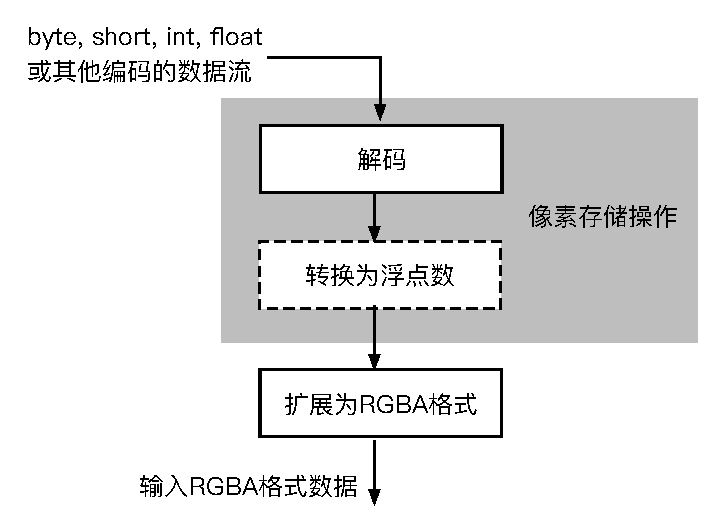
\includegraphics[width=0.65\textwidth]{figures/api/unpack}
	\caption{OpenGL中纹理数据由客户内存传输到设备内存中的解码过程。}
	\label{f:api-unpack}
\end{figure}

转换为浮点数的过程是可选的,着色器仍然可以选择使用整数采样器来获取原始的整数值。最后,不管内部格式的分量数量多少,读进着色器中的值都会被扩展为RGBA4个分量的格式,如果内部格式不包含A分量,则当输出为浮点数时A分量为1.0,否则为1;如果不包含R,G或B中的任意一个分量,则根据输出数据类型是否为浮点型其值为0.0(浮点数时)或0(整数时)。

以上这些参数仅仅只能表述单个纹素的的布局结构,OpenGL还提供了其他一些参数来控制像素数据的传输,这些参数可以通过以下命令来设置:

\begin{lstlisting}[language=C++]
void glPixelStoref(GLenum pname​, GLfloat param​);
void glPixelStorei(GLenum pname​, GLint param​);
\end{lstlisting}

这些命令影响大部分像素数据的编码和解码操作,其中pname表示各个参数的名称,param表示参数设置的值,pname的名称具有GL\_PACK\_或GL\_UNPACK\_作为前缀以分别对应像素编码和解码操作。这些参数可以用来设置整体传输数据的布局,例如可以只传输目标纹理一部分子区域的数据,如图\ref{f:api-pixel-store}所示。

\begin{figure}
\sidecaption
	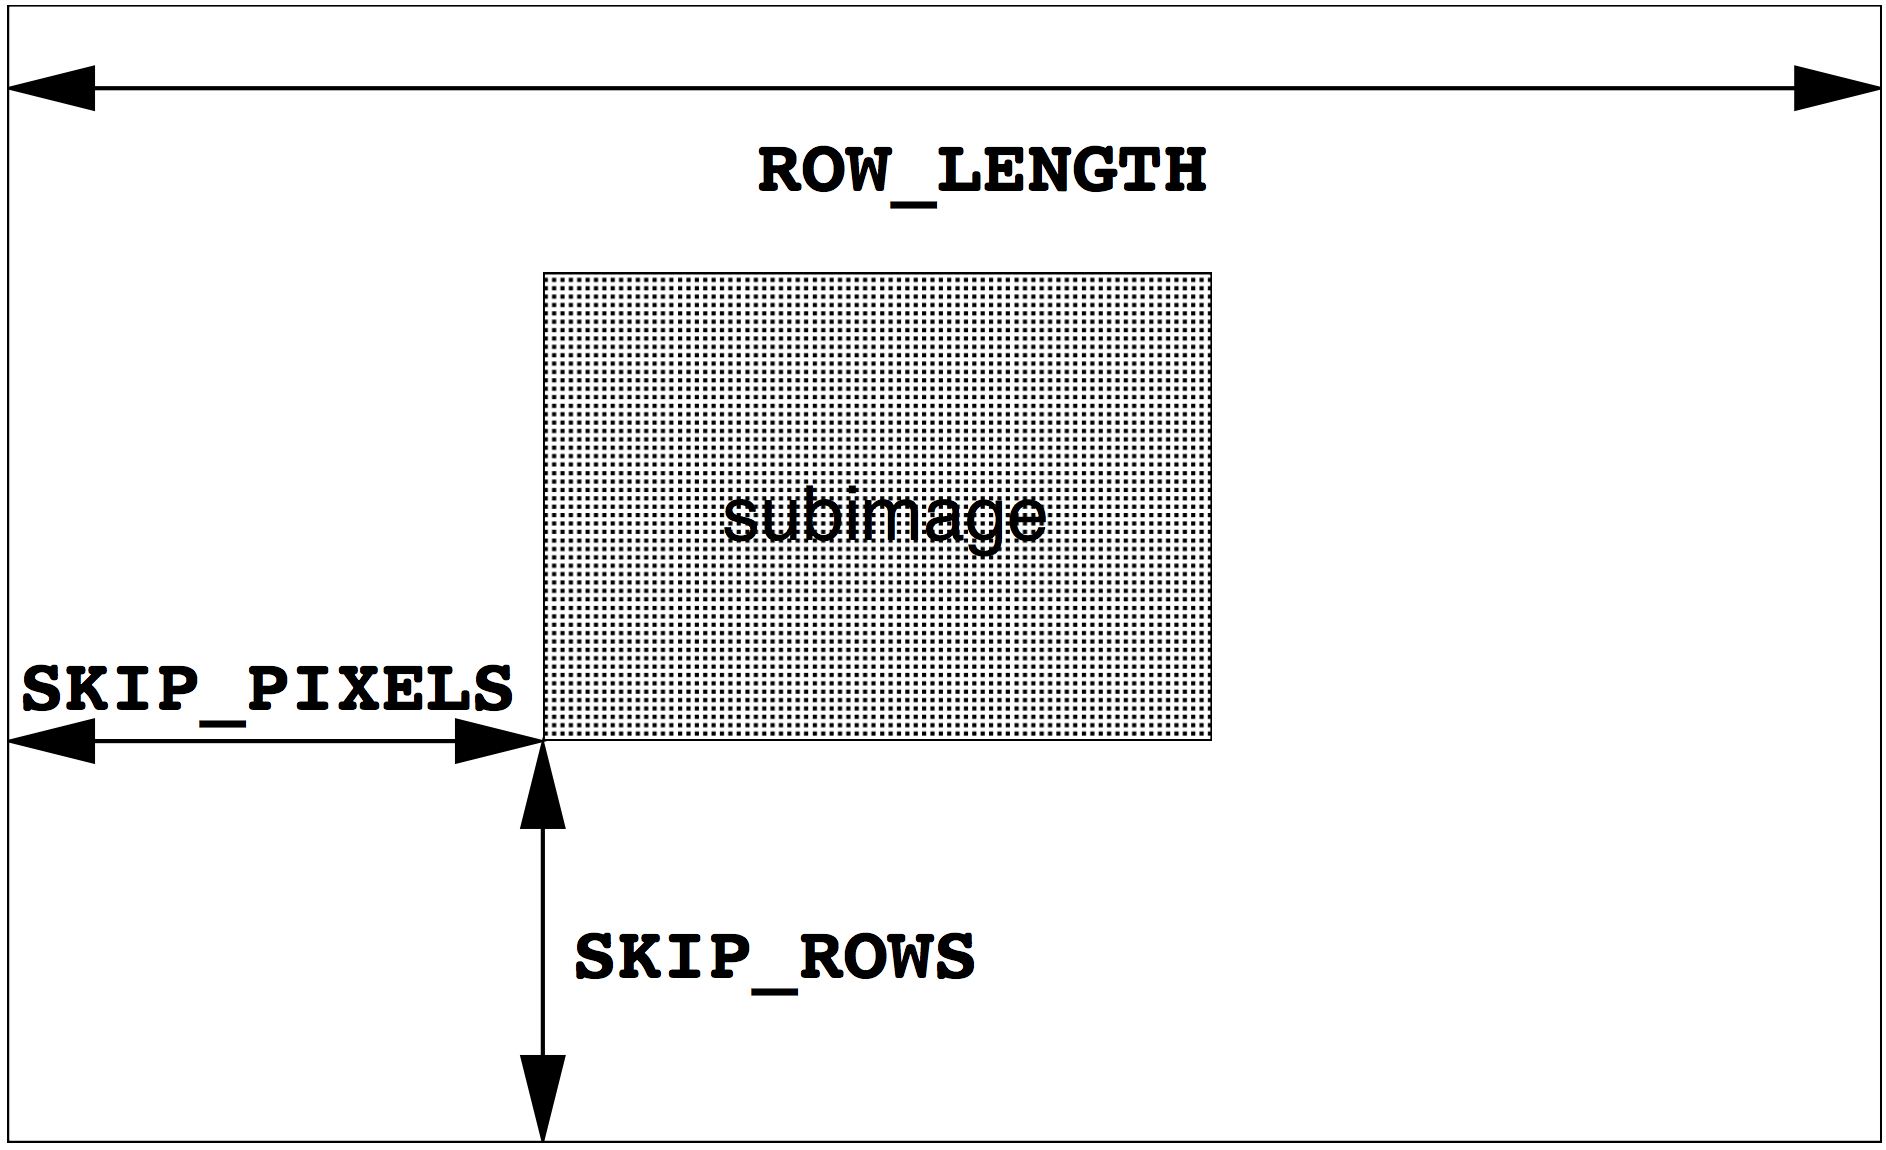
\includegraphics[width=0.6\textwidth]{figures/api/PixelStore}
	\caption{从一个图形传输一个子区域,这些参数的名称以前缀UNPACK\_(针对TexImage*)和PACK\_(针对ReadPixels)开头。}
	\label{f:api-pixel-store}
\end{figure}





\subsection{压缩纹理}\label{sec:api-compressed-texture}
在3D图形程序中,纹理不仅占据了大量的应用程序资源内容,也占据了大量的运行时内存使用,传统的压缩方案如JPG能够减小资源的大小,但并不能对内存有多大贡献,通过前面的内容我们知道一个图形数据在被传输到OpenGL服务端内存时,都需要被转化为RGB或者RGBA未压缩的格式,这才能保证实时渲染的性能,OpenGL并不识别一般的压缩算法。因此需要一种新的针对GPU的纹理压缩方案。

1996年,斯坦福大学的Andrew Beers,Maneesh Agrawala和Navin Chaddha共同发表了一篇论文\cite{a:RenderingfromCompressedTextures},提出了一种基于GPU的纹理压缩方法,该方法使得GPU可以直接从压缩纹理中采样进行渲染。由于纹理在设备内存中以压缩格式存在,所以此方法不仅能减少资源的大小,同时能减少内存的占用。

\subsubsection{压缩纹理的特点}
在这篇论文中提出纹理压缩技术相较于其他图像压缩技术(如JPG)具有以下4个方面的特征:

\begin{itemize}
	\item 解压速度快:为了使渲染系统可以直接从压缩纹理中读取数据,该压缩技术必须具有快速的解压速度,以不影响渲染系统的性能。传统的压缩技术主要针对存储或者文件传输的需求的进行设计,并不具备快速的解压速度。
	\item 随机读取:由于纹理中的任何位置可能会被图元映射,因此片元着色器可能随机读取纹理中任何位置的纹素,这就要求该压缩技术必须能够被随机读取。传统的压缩技术如JPEG使用可变的压缩比率,读取某个像素的信息可能要解压很大一部分相关的像素信息。压缩纹理技术则使用固定的压缩比率,访问纹素时可以根据索引快速读取某一小块的内容,从而可以高效地实现随机读取。
	\item 压缩率和图像质量:传统的图像压缩技术,大多要考虑图像的质量,因为这些压缩图像自身会作为一个整体被查看和使用。而对于纹理压缩技术,每个纹理只是场景的一部分,整体场景渲染质量的重要性大于单个图片的质量重要性,所以压缩纹理通常使用有损压缩\footnote{无损压缩通常用于数据文件,它们需要被精确恢复;而有损压缩通常用于一些表示函数的采样数据,这样的数据本身是包含噪声,并且在一定范围内人是无法感知的,例如声音,视频,图像等文件。}。
	\item 编码速度:压缩纹理的压缩过程通常发生在应用程序之外,因此并不需要较高的编码速度,使用压缩纹理的核心制约因素是解压速度。

\end{itemize}

满足上述特点的纹理压缩方法,不仅可以减小图像资源的大小,还可以配合GPU进行高效渲染,从而大大减少内存占用。压缩纹理同时减少了应用程序客户端向GL服务端传输纹理数据的带宽,由于减小内存以及其直接存储在GPU中因此芯片可以对其进行更高效的使用,从而可以减少移动设备电量的消耗。 另外,在OpenGL中,压缩纹理同其他纹理一样进行采样,支持多级纹理等,应用程序除了通过特殊的glCompressedTexImage*来传输纹理,其他方面和普通纹理几乎没有什么区别。



\subsubsection{压缩纹理的实现}
为了达到上述这些要求和特征,压缩纹理使用一种特殊的方式来实现纹理的压缩和解压,关于压缩纹理更详细的算法和原理超出本书的范畴,这里仅讲述压缩纹理的随机读取的大概思路,以使读者对压缩纹理有更直观的理解。此外,有些压缩纹理格式如PVRTC使用不同的压缩和读取算法。

传统的图像压缩算法为了保证最大的压缩比,使用一个可变的压缩比率,这就要求在解压的时候要解压更多的像素位才能读取某个像素的位置,这对于随机和快速读取都是不利的,实际上传统的图像压缩算法都是为了存储,传输等目的而设计,而不是为了实时渲染。

所以,压缩纹理使用一个固定的压缩比率,它首先按照这个比率将纹理分成很多的像素块(block),每个像素块包含如2$\times$2或4$\times$4个像素,然后对每个像素块进行压缩。每个被压缩后的像素信息存储在一个像素块集合(Codebook)\index{像素块集合codebook}\index[en]{codebook像素块集合}中,而一个块索引图(Index Map)存储了每个x=像素块的索引位置,在读取的时候首先根据块索引找到像素块,然后解压该像素块读取偏移值的信息。这称作为基于块(block-based)的压缩算法,如图\ref{f:api-compression}所示。

\begin{figure}
\begin{center}
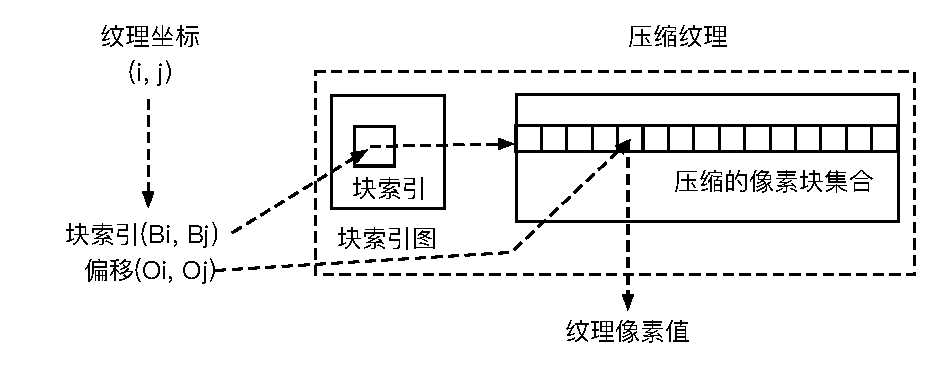
\includegraphics[width=0.81\textwidth]{figures/api/compression}
\end{center}
	\caption{压缩纹理使用固定的压缩比率进行压缩,一个固定大小的块内的像素被压缩以便于快速读取。}
	\label{f:api-compression}
\end{figure}

例如图\ref{f:api-compression}的像素读取过程可以描述为:

\begin{enumerate}
	\item 首先将纹理坐标转化为块索引值,并计算出块索引值,以及该坐标在该像素块内的偏移值。
	\item 根据块索引值在像素块集合(Codebook)中查找对应的像素块。
	\item 在这一段像素块中查找纹理坐标$(i,j)$的颜色值。
\end{enumerate}

通过对固定数量的像素块进行压缩,压缩纹理就能够更快速的读取,实际在操作的时候对于一个像素块的数据还可以根据实际情况进行缓存。这种快速解压的速度使得图形渲染管线可以不依赖于CPU的解压就可以实现实时渲染,将压缩纹理直接保存在GPU内存中,既减少了资源在磁盘的存储大小,也大大节省了内存占用,还减少了纹理在传输过程中所占用的带宽。





\subsubsection{在OpenGL中使用压缩纹理}
在OpenGL中使用压缩纹理有两种方法,一种是让OpenGL为我们压缩,在这种情况下,使用前面讲述的数据存储分配方法glTexImage*提供未压缩的原始纹理数据,同时指定纹理内部格式为表\ref{t:api-compression-internal-format}中的压缩纹理格式,这样OpenGL将会为我们实现纹理压缩。由于这是一个实时的过程,为了保证速度,OpenGL实现的压缩算法导致的纹理精度可能很低。另外一种是使用一些离线工具把纹理数据提前压缩好,然后直接传递压缩过的纹理数据给OpenGL,使用这种方法,我们可以花费更多的时间来获取更好的压缩质量,而不需要牺牲运行时时间。

需要注意的是,表\ref{t:api-compression-internal-format}中的很多格式是由OpenGL扩展支持的,所以在实践中我们需要首先查询不同的OpenGL实现支持哪些扩展的压缩纹理格式。


\begin{table}
\caption{客户内存中的像素数据的类型,以及对于的GL类型}
\label{t:api-compression-internal-format}
\centering
\begin{tabular}{>{\small}p{0.5\textwidth}|>{\small}p{0.16\textwidth}|>{\small}p{0.16\textwidth}|>{\small}p{0.15\textwidth}}
\hline 
   压缩纹理内部格式:COMPRESSED\_* & 基本内部格式 & 类型 & 边界类型\\
    \hline  
    RED                         &  RED   &  一般   &unorm\\
    RG                          &  RG    &  一般   &unorm\\
    RGB                         &  RGB   &  一般   &unorm\\
    RGBA                        &  RGBA  &  一般   &unorm\\
    SRGB                        &  RGB   &  一般   &unorm\\
    SRGB\_ALPHA                 &  RGBA  &  一般   &unorm\\
    RED\_RGTC1                  &  RED   &  特殊   &unorm\\
    SIGNED\_RED\_RGTC1          &  RED   &  特殊   &snorm\\
    RG\_RGTC2                   &  RG    &  特殊   &unorm\\
    SIGNED\_RG\_RGTC2           &  RG    &  特殊   &snorm\\
    RGBA\_BPTC\_UNORM           &  RGBA  &  特殊   &unorm\\
    SRGB\_ALPHA\_BPTC\_UNORM    &  RGBA  &  特殊   &unorm\\
    
    RGB\_BPTC\_SIGNED\_FLOAT    &  RGB   &  特殊   &float\\
    RGB\_BPTC\_UNSIGNED\_FLOAT  &  RGB   &  特殊   &float\\
    RGB8\_ETC2                  &  RGB   &  特殊   &unorm\\
    SRGB8\_ETC2                 &  RGB   &  特殊   &unorm\\
    RGB8\_PUNCHTHROUGH\_ALPHA1\_ETC2  &  RGB  &  特殊   &unorm\\
    SRGB8\_PUNCHTHROUGH\_ALPHA1\_ETC2 &  RGB  &  特殊   &unorm\\
    SRGB8\_ETC2\_EAC            &  RGBA  &  特殊   &unorm\\
    SRGB8\_ALPHA8\_ETC2\_EAC    &  RGBA  &  特殊   &unorm\\
    R11\_EAC                    &  RED   &  特殊   &unorm\\
    R11\_SIGNED\_R11\_EAC       &  RED   &  特殊   &snorm\\
    RG11\_EAC                   &  RG    &  特殊   &unorm\\
    SIGNED\_RG11\_EAC           &  RG    &  特殊   &snorm\\

 \hline 
\end{tabular}
\end{table}

如果使用的是已压缩好的纹理数据,则需要使用另外的纹理存储分配函数,分配可改变的压缩纹理可以使用如下命令:

\begin{lstlisting}[language=C++]
void glCompressedTexImage1D(GLenum target, GLint level, GLenum internalFormat, GLsizei width, GLint border, GLsizei imageSize, const void *data);
void glCompressedTexImage2D(GLenum target, GLint level, GLenum internalFormat, GLsizei width, GLsizei height, GLint border, GLsizei imageSize, const void *data);
void glCompressedTexImage3D(GLenum target, GLint level, GLenum internalFormat, GLsizei width, GLsizei height, GLsizei depth, GLint border, GLsizei imageSize, const void *data);
\end{lstlisting}

如果需要分配不可改变的存储,仍然使用前面的glTexStorage*命令来分配存储,然后使用相应的glCompressedTexSubImage*类函数来更新(而不是改变)纹理存储内的数据。






\subsection{采样器对象}
纹理是一个分布函数,当我们在获取某个位置的纹素时,需要对其进行重采样,所以着色器中获取到的通常并不一定是纹理中的真实数据。为了支持这种采样操作,纹理对象需要设置一些采样相关的参数。

\begin{figure}
\sidecaption
	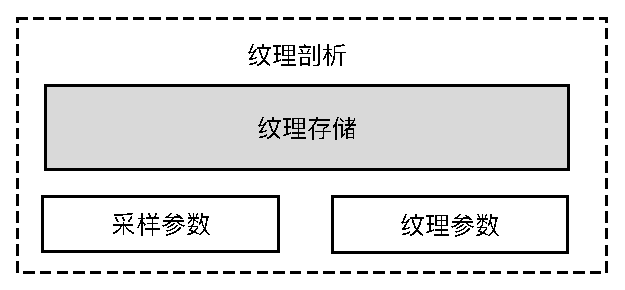
\includegraphics[width=0.6\textwidth]{figures/api/texture-anatomy}
	\caption{一个纹理对象的状态可以分为两个部分:与纹理尺寸,维度,图像等相关的状态,以及与采样相关的状态。}
	\label{f:api-sampler-parameter}
\end{figure}

在OpenGL中,一个纹理对象实际上包含两个类别的参数(或者状态):第一个类别表示纹理的尺寸,维度以及其他图像相关的参数,第二个类别则是采样相关的参数,如图\ref{f:api-sampler-parameter}所示。所有的这些参数都可以通过以下这些命令(仅列出部分)设置:

\begin{lstlisting}[language=C++]
void glTexParameter{if}( GLenum target​, GLenum pname​, T param​);
void glTexParameter{if}v​(GLenum target​, GLenum pname​, T *params​);
\end{lstlisting}

本节我们仅讨论采样相关的参数,纹理对象的采样参数可以被用一个专门的采样器对象来表述,一个采样器对象包含全部采样相关的参数。一个采样器对象(Sampler object)\index{采样器对象sampler object}\index[en]{sampler object采样器对象}是一个标准的OpenGL对象,它使用glGenSamplers, glDeleteSamplers命令来创建和删除,并使用glBindSampler命令来绑定采样器对象到某个纹理单元,不同的是它可以同时被绑定到多个纹理单元上。

当创建采样器对象之后,我们就可以使用以下命令(同样仅包含部分)来设置采样参数:

\begin{lstlisting}[language=C++]
void SamplerParameter{if}( uint sampler, enum pname, T param );
void SamplerParameter{if}v( uint sampler, enum pname, const T* param);
void SamplerParameterI{i ui}v( uint sampler, enum pname, const T* params);
\end{lstlisting}

这里pname表示参数名称,param和params分别用来设置单个值的参数和数组值的参数。采样器参数名称的可选值包括:GL\_TEXTURE\_WRAP\_S, GL\_TEXTURE\_WRAP\_T, GL\_TEXTURE\_WRAP\_R, GL\_TEXTURE\_MIN\_FILTER, GL\_TEXTURE\_MAG\_FILTER, GL\_TEXTURE\_MIN\_LOD, GL\_TEXTURE\_MAX\_LOD, GL\_TEXTURE\_LOD\_BIAS, GL\_TEXTURE\_COMPARE\_MODE和GL\_TEXTURE\_COMPARE\_FUNC。以下按类别分别讲述这些参数。

采样器最重要的参数是用来对离散函数进行重采样的滤波器的设置,这包括信号的放大和缩小。对于放大过滤器(Magnification filter)\index{放大过滤器magnification filter}\index[en]{magnification filter放大过滤器},其对应的参数名称为 GL\_TEXTURE\_MAG\_FILTER,可选的值为GL\_LINEAR和GL\_NEAREST,分别表示使用线性插值和使用最近点作为采样值;对于缩小过滤器(Minification filter)\index{缩小过滤器minification filter}\index[en]{minification filter缩小过滤器},采样参数的设置还涉及mipmap的选择,我们可以选择不使用更小的mipmap级别,或者我们也可以选择对mipmap进行采样(插值),这些可选的值如表\ref{t:api-minification-filter}所示。

\begin{table}
\caption{OpenGL中的缩小滤波器的可选值及其意义}
\label{t:api-minification-filter}
\centering
\begin{tabular}{>{\small}p{0.5\textwidth}|>{\small}p{0.16\textwidth}|>{\small}p{0.16\textwidth}|>{\small}p{0.15\textwidth}}
\hline 
   参数值 & 是否在mipmap内部线性插值 & 是否使用mipmap & 是否mipmap之间线性插值\\
    \hline  
    GL\_NEAREST                  &  否   &  否   &\\
    GL\_LINEAR                   &  是   &  否   &\\
    GL\_NEAREST\_MIPMAP\_NEAREST &  否   &  是   &否\\
    GL\_LINEAR\_MIPMAP\_NEAREST  &  是   &  是   &否\\
    GL\_NEAREST\_MIPMAP\_LINEAR  &  否   &  是   &是\\
    GL\_LINEAR\_MIPMAP\_LINEAR   &  是   &  是   &是\\

 \hline 
\end{tabular}
\end{table}

这些值的意义可以参见第一章的内容,需要注意的是,纹理的重采样是硬件支持的功能,它们能够高效地满足着色器的随机存储,这也是纹理对象和一般缓存对象不同的地方。

采样器的另一些参数用来控制存储深度值的纹理的比较模式(Comparison mode)\index{比较模式comparison mode}\index[en]{comparison mode比较模式}。如果纹理是用来存储的深度值,通常它的作用是用来进行深度比较(就像OpenGL自身对深度缓存的使用方式),所以当我们想要对一个深度纹理进行采样时,往往我们并不是希望获取它作为一个纹理的纹素值,而是希望获取一个它与某个参考值进行比较的结果作为采样值。跟OpenGL渲染管线本身的深度比较一样,我们需要设置一个比较模式(GL\_TEXTURE\_COMPARE\_MODE参数)和一个比较函数(GL\_TEXTURE\_COMPARE\_FUN参数)同时来进行工作,由于它和渲染管线深度比较的工作方式一致,我们将在本章后面讲述深度比较的方法。此外,存储深度值的纹理也可以像一般纹理那样使用滤波器获取一个普通的采样值。

使用一些采样器参数用来控制对边缘值的采样(Edge value sampling),虽然纹理坐标使用归一化的值其范围在0.0和1.0之间,但是OpenGL并不阻止其使用该范围以外的浮点值,这有时候是非常有用的。当一个纹理坐标的值超出[0,1]的范围时,OpenGL需要知道该怎样进行采样。

纹理坐标的每个维度都可以分别设置不同的边缘采样模式,参数GL\_TEXTURE\_WRAP\_S, GL\_TEXTURE\_WRAP\_T, 和 GL\_TEXTURE\_WRAP\_R分别用来设置纹理坐标S, T和 R轴的值,这些可选的值包括:

\begin{itemize}
	\item GL\_REPEAT: 纹理坐标缠绕着纹理,比如纹理坐标为$-0.2$时相当于其坐标为0.8。	
	\item GL\_MIRRORED\_REPEAT: 纹理坐标以镜面的形式围绕纹理缠绕,例如纹理坐标为$-0.2$时等效于纹理坐标为0.2,当纹理坐标为$-1.2$时等效于纹理坐标为0.8。
	\item GL\_CLAMP\_TO\_EDGE: 所有纹理坐标被限制在[0,1]范围,即所有纹理坐标大于1时为1,小于0时为0。
	\item GL\_CLAMP\_TO\_BORDER: 所有纹理坐标被限制在[0,1]的范围,但是边缘的纹理值将是和一个常数值进行混合的结果。
	\item GL\_MIRROR\_CLAMP\_TO\_EDGE: 纹理坐标被限制在$[-1,1]$的范围,但是负数部分与正数部分呈镜面对称,所以它的结果使整个纹理以镜面的形式两倍于原纹理大小。
\end{itemize}

同样需要注意的是,对纹理边缘的采样控制仍然是基于硬件实现的。





\subsection{特殊纹理}
本节讨论一些特殊用法的纹理,这些纹理中每个图像的内部格式都遵循前面讲述的基本内容,但是它们在整体结构上有一些差异,对这些结构的特殊处理都集成在硬件内部,从而使这些复杂的纹理应用场景得以简化。

\subsubsection{立方体纹理}
传统的1D,2D和3D纹理所代表的分布函数都是针对空间域的,即这些纹理中每个纹素代表的是一维,二维和三维空间域中的某个位置的值\footnote{当然2D纹理所代表的空间域通常并不仅仅是一个平面空间,它往往是把一个3D物体的不平整的表面展开在一个2D的平面空间上。}。

显然,如果使用3D纹理存储一个三维空间的的某种分布数据(如颜色值),这将是一个巨大的挑战,所以在本书后面的内容我们将看到,游戏开发或其他图形应用程序中往往并不会直接使用3D纹理存储完整的空间分布。对于3D空间域的分布函数,我们往往需要分析其分布函数的特征,然后考虑能不能以其他更低空间域(例如2D甚至1D)或更低的分辨率来表示,例如本书后面将会讨论的一些3D空间的分布函数具有较低的频率域(如间接光),因此可以使用很低的分辨率来存储这些值,另一些3D分布函数存在大量的空值,则可以使用一些特殊的数据结构来使3D纹理仅仅被用来保存一些局部信息。

立方体纹理(Cubemap texture)\myindex{立方体纹理}{cubemap texture}就是一种特殊的3D分布函数。我们发现,对于物体周围的反射光源,如果这些环境离观察点的距离很远,那么观察点的位置对反射光的影响可以忽略不计,因此3D空间分布被简化为一个方向分布,我们可以使用任意一种能够包括全部方向的一个“薄面”结构来代替这种3D分布,例如一个球体,一个立方体,或者任意其他能够包围一个环境的结构。球体显然是最理想的选择,但是立方体具有更简单的采样方式因此被一般的图形硬件支持。

\begin{figure}
\sidecaption
	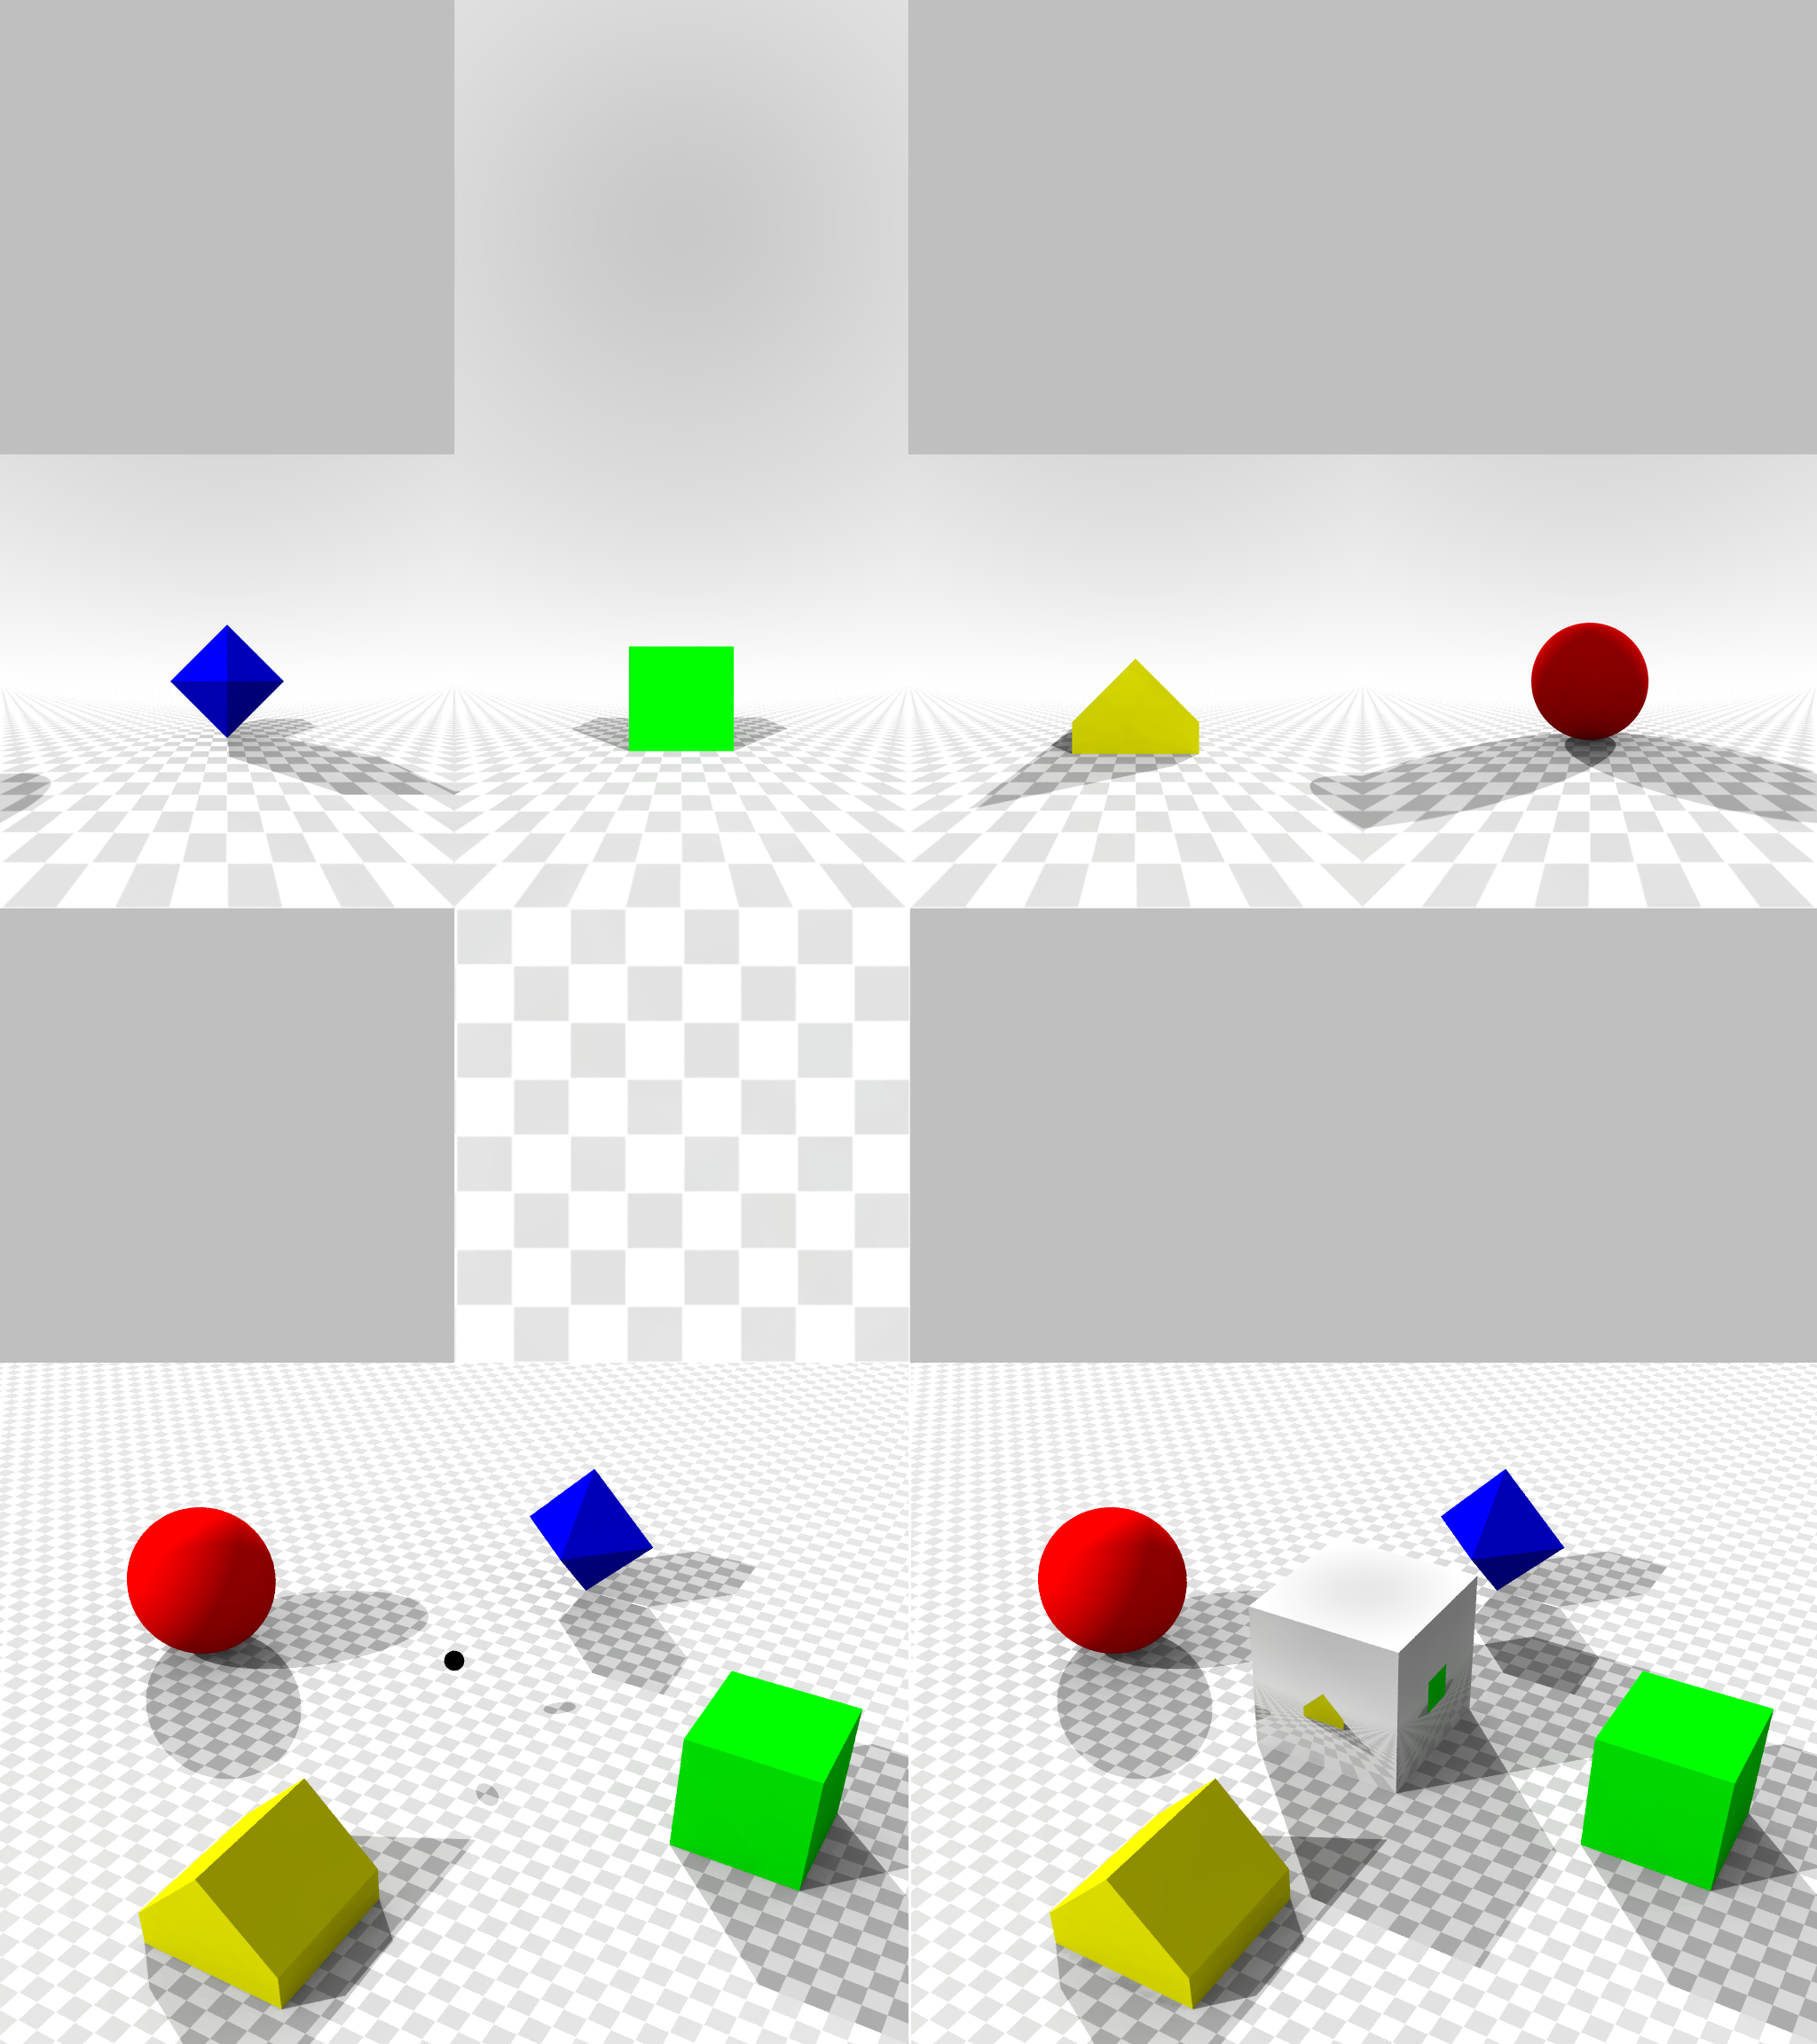
\includegraphics[width=0.65\textwidth]{figures/api/cube-map}
	\caption{左下角的图表示原始场景,将观察点置于场景中的小黑点的位置。上面的图表示从观察点渲染或者看到的6个方向的2D图像,它们形成立方体纹理的6个面。最后右下角的场景中,新加入的中间的白色立方体使用前面的立方体纹理对其进行环境映射,就是该物体看起来可以反射周围的环境(图片来自Wikipedia)。}
	\label{f:api-cube-map}
\end{figure}

使用立方体可以很方便地构造环境分布函数,对于环境光来说,只需要将摄像机放置于环境中央,然后正对立方体的6个面分别执行一次普通的渲染工作,这6个面分别用一个等大小的2D纹理来存储颜色数据,如图\ref{f:api-cube-map}所示。

立方体纹理对象的绑定目标为GL\_TEXTURE\_CUBE\_MAP,但是立方体纹理的存储和数据分配使用一种特殊的方式,即它的数据传输命令中的每个目标需要分别设置每一个面所代表的一个特殊的目标,这6个面的目标值分别是:GL\_TEXTURE\_CUBE\_MAP\_POSITIVE\_X, GL\_TEXTURE\_CUBE\_MAP\_NEGATIVE\_X, GL\_TEXTURE\_CUBE\_MAP\_POSITIVE\_Y, GL\_TEXTURE\_CUBE\_MAP\_NEGATIVE\_Y, GL\_TEXTURE\_CUBE\_MAP\_POSITIVE\_Z以及 GL\_TEXTURE\_CUBE\_MAP\_NEGATIVE\_Z。

立方体6个2D的面都有自己的mipmap,这跟一般的2D纹理一样可以通过glTexImage2D来设置。立方体纹理的采样器使用gsamplerCube或gsamplerCubeShadow类型,这里g代表立方体纹理中的数据类型,可以是i(有符号),ui(无符号)或f(浮点数),立方体纹理坐标是一个3D的矢量,其表示一个方向,所以立方体的纹理坐标不一定需要归一化。gsamplerCubeShadow的纹理坐标是一个4D的矢量,其第四个分量表示进行深度比较的一个比较值。

使用立方体纹理对环境进行映射的一个缺点是,6个面之间的连接处会存储不连续的缺陷。传统的纹理滤波器技术只在每个2D纹理内部工作,而不能对这种情况进行处理。但是现代的硬件能够直接在相邻的纹理间进行插值,这可以通过以下设置来使用这种特性:

\begin{lstlisting}[language=C++]
glEnable(GL_TEXTURE_CUBE_MAP_SEAMLESS)​;
\end{lstlisting}

此外,在本书后面的具体例子中,还会介绍一些其他的方法来解决立方体纹理每个面之间映射不连续的情况。
 




\subsubsection{数组纹理}
数组纹理(Array texture)是指在纹理的每个mipmap层级内包含的是一个图像或图像集(即纹理包含多个图像)的数组,而不是单个图像或图像集。我们称该数组中的一个元素为一个纹理切片(Texture layer)\index{纹理切片texture layer}\index[en]{texture layer纹理切片},由此可见,从图像数量上看,一个切片数量为$n$的数组纹理等效于一个其下一个更高维维度的尺寸为$n$的纹理,例如一个切片数为5的2D数组纹理,其图像数量与深度为5的一个3D纹理一致。

但是数组纹理与下一个更高维度的纹理在使用上有很大的区别,例如对一个3D纹理进行采样,对深度的选择的坐标将被归一化,然后使用滤波器对深度进行采样,而数组纹理则使用一个整数来选择切片。

数组纹理适用于在一次绘制中需要用到多种同等尺寸的纹理,例如对一个角色使用多层纹理(散射颜色,法线贴图等具有相同尺寸的纹理),或者多个不同的角色使用不同的皮肤等,这些纹理可以存储为一个数组纹理,在贴图的时候可以独立选择任意一个单独纹理(切片)。

数组纹理的基础类型只能来自于1D,2D或立方体纹理,其对应的绑定目标类型分别为GL\_TEXTURE\_1D\_ARRAY,GL\_TEXTURE\_2D\_ARRAY和GL\_TEXTURE\_CUBE\_MAP\_ARRAY。数组纹理也可以具有mipmap,但是每个切片具有的mipmap的级数必须相等。此外,数组纹理数据的分配方式需要使用其下一个更高维度对应的数据分配命令,例如一个2D的数组纹理需要使用3D纹理的数据分配命令:


\begin{lstlisting}[language=C++]
glBindTexture(GL_TEXTURE_2D_ARRAY, tex);
glTexImage3D(GL_TEXTURE_2D_ARRAY, 0, format, width, height, num_layers, ...);
glTexImage3D(GL_TEXTURE_2D_ARRAY, 1, format, width/2, height/2, num_layers, ...);
glTexImage3D(GL_TEXTURE_2D_ARRAY, 2, format, width/4, height/4, num_layers, ...);
\end{lstlisting}

其中,3D纹理的深度被2D数组纹理的切片数num\_layers代替。数组纹理拥有独立不同的采样器类型,其分别为gsampler1DArray​, gsampler2DArray​以及gsamplerCubeArray,这些采样器相较于其基本类型的采样器,它们会使用一个额外的整数参数来选择切片。​





\section{帧缓存}\label{sec:api-framebuffer}
帧缓存(Framebuffer)\index{帧缓存framebuffer}\index[en]{framebuffer帧缓存}是OpenGL渲染管线的最终目标,由于我们使用图形渲染管线的目的是得到一张2D图像,因此不难想象帧缓存是由一个2维的矩形像素数组构成的图像,它的分辨率和当前设备的(或部分)显示分辨率一致。因此我们想要得到任何渲染结果,都必须通过帧缓存对象,这包括提交图像给输出设备显示,或者读取渲染结果回宿主程序供其他使用目的(如制作视频流)。

在OpenGL中,帧缓存对象分为两种类别,虽然它们的内部结构很相似,但是它们的使用差别有很大不同。第一种称为默认帧缓存(Default framebuffer),它是由宿主程序在创建OpenGL上下文的时候形成,默认帧缓存仅供显示使用,应用程序不能做太多控制;相反,第二种应用程序创建的帧缓存(Application-created framebuffer)完全受应用程序控制,但是它的渲染结果不能直接被显示,它可以用于将渲染结果保存到纹理对象,甚至用于离线渲染将渲染结果保存回宿主供其他使用。随着延迟渲染等渲染方法的兴起,一次完整的渲染往往需要使用多次渲染管线(或计算着色器)的计算,应用程序创建的帧缓存被大量使用以用来将一些中间过程计算结果保存到纹理中,最终才将最后的计算结果显示出来。为了简化,在以下的内容中,我们将直接称应用程序创建的帧缓存为帧缓存。

帧缓存对象是一个普通的OpenGL对象,因此我们仍然使用一般的glGenFramebuffers和glDeleteFramebuffers来创建和删除帧缓存对象,并使用glBindFramebuffer来绑定要使用的帧缓存对象到当前上下文。帧缓存的绑定目标有三个:GL\_FRAMEBUFFER, GL\_READ\_FRAMEBUFFER和GL\_DRAW\_FRAMEBUFFER,其中GL\_READ\_FRAMEBUFFER将帧缓存绑定为一个只读的对象,而GL\_DRAW\_FRAMEBUFFER可以接受所有绘制命令(包括清除),如果我们希望同时可以执行两种操作\footnote{GL\_READ\_FRAMEBUFFER可以用来防止在复制数据到客户内存(或其他缓存对象)期间帧缓存数据被其他绘制命令修改。},则使用GL\_FRAMEBUFFER。

上述我们假想的认为“一个帧缓存包含一个2D的图像”并不对,帧缓存实际上是一个容器对象,它包含多个具有相同尺寸的2D图像。帧缓存以附加点(Attachment points)\index{附加点attachment points}\index[en]{attachment points附加点}的方式让应用程序可以管理这些2D图像,应用程序可以把一个对应的可附加的对象附加到这些附加点,这些附加点的名称可以分为4类,分别用来存储颜色,深度,模板值,如表\ref{t:api-attachment-points}所示,其中具有多个用来储存颜色的附加点。

\begin{table}
\caption{帧缓存附加点,其中GL\_COLOR\_ATTACHMENT$i$中的$i$的取值范围从0到GL\_MAX\_COLOR\_ATTACHMENTS之间,所有OpenGL实现保证GL\_MAX\_COLOR\_ATTACHMENTS的最小值为8。}
\label{t:api-attachment-points}
\centering
\begin{tabular}{>{\small}p{0.53\textwidth}|>{\small}p{0.44\textwidth}}
\hline 
   附加点名称 & 缓存名称\\
    \hline  
    GL\_COLOR\_ATTACHMENT$i$       &颜色缓存\\
    GL\_DEPTH\_ATTACHMENT          &深度缓存\\
    GL\_STENCIL\_ATTACHMENT        &模板缓存\\
    GL\_DEPTH\_STENCIL\_ATTACHMENT &深度模板缓存\\

 \hline 
\end{tabular}
\end{table}

这些2D图像被称为一个缓存对象,它们的名字如表\ref{t:api-attachment-points}所示。对于默认帧缓存,它的颜色缓存最多可以包含4个,分别是GL\_FRONT\_LEFT, GL\_BACK\_LEFT, GL\_FRONT\_RIGHT和GL\_BACK\_RIGHT,即所谓的双缓存(Double-buffered),其中GL\_FRONT*通常是表示显示在屏幕上的帧缓存,而GL\_BACK*则表示渲染管线正在使用的帧缓存,它们通过相互交换来实现在屏幕上的显示。*\_LEFT和*\_RIGHT用来支持3D的立体渲染(Stereoscopic rendering)\index{立体渲染stereoscopic rendering}\index[en]{stereoscopic rendering立体渲染},它需要包含左右两个镜头的图像数据,如果只是普通的渲染,则一般使用*\_LEFT颜色缓存。

这些缓存对象具有内部格式用于指示其图像中像素的存储结构,这些内部格式是纹理内部格式的一个子集(不包含压缩纹理)。所有缓存中的每个像素最多具有4个分量,分别表示R,G,B以及A分量,每个分量的数据类型可以是有符号或无符号的归一化的浮点数,或者有符号或无符号的整数,但是所有分量必须具有相同的类型和表述。深度缓存中的每个像素可以是一个无符号的整数值或浮点值,模板缓存中的每个像素是一个无符号的整数值。

在OpenGL中,可被附加到帧缓存的每个附加点的对象类型有两种:渲染缓存或纹理。它们都可以用来实现离线渲染,即将渲染结果读回到客户内存中,在这方面,渲染缓存是一个更好的被优化的渲染目标;然而当渲染结果需要被着色器重采样(被着色器读取)时,则只能选择渲染到纹理中。

渲染缓存(Renderbuffer)\index{渲染缓存renderbuffer}\index[en]{renderbuffer渲染缓存}对象是一个OpenGL对象,它使用glGenRenderbuffers和glDeleteRenderbuffers​来创建和删除一个渲染缓存对象,并使用glBindRenderbuffer来绑定渲染缓存对象,其绑定的目标必须是GL\_RENDER- BUFFER。

渲染缓存使用以下命令来分别存储:

\begin{lstlisting}[language=C++]
void glRenderbufferStorage​(GLenum target​, GLenum internalformat​, GLsizei width​, GLsizei height​);
void glRenderbufferStorageMultisample​(GLenum target​, GLsizei samples​, GLenum internalformat​, GLsizei width​, GLsizei height​);
\end{lstlisting}

其中,internalformat表示渲染缓存的内部格式,它遵循帧缓存可附加对象内存格式的要求,glRenderbufferStorageMultisample用来实现多重采样。注意,和纹理对象不一样,渲染缓存不需要分配初始数据,渲染缓存的数据只能被渲染管线写入。

渲染缓存使用以下命令附加到帧缓存的一个附加点:

\begin{lstlisting}[language=C++]
void FramebufferRenderbuffer( enum target, enum attachment, enum renderbuffertarget, uint renderbuffer );
\end{lstlisting}

这里target是GL\_DRAW\_FRAMEBUFFER, GL\_READ\_FRAMEBU- FFER或FRAMEBUFFER,renderbuffertarget必须是GL\_FRAMEBUFFER,renderbuffer是渲染缓存的名称,attachment是帧缓存的一个附加点名称。实际上,在OpenGL中渲染缓存唯一被使用的方式就是被附加到一个帧缓存对象上。

对于纹理对象的附件,由于帧缓存中的每个附加点只存储一个2D图像,并且纹理实际上是一个图像的集合,此外,纹理还可能拥有多个级别的mimap,所以有一些规则用来限制纹理的绑定,这些规则如下:

\begin{itemize}
	\item 当一个1D纹理被附加到帧缓存时,它被当做一个2D的图像,其垂直高度为1。1D纹理中的每个图像可以用一个mipmap的级别表示\footnote{纹理对象在结构上虽然可以由多个图像构成,但是图像的数量其实是由OpenGL控制的,而不是由应用程序控制的,例如1D和2D纹理的每个mipmap级别都只有1个图像,立方体纹理每个级别固定有6个图像。}。
	\item 2D纹理中的图像则可以被正常使用,其每个图像可以用mipmap级别唯一表示。
	\item 3D纹理被认为是一个2D纹理的集合,其Z轴(或深度)中的每个整数索引被认为是一个层(layer),在附加的时候需要指定使用哪一层级,同样立方体纹理也需要指定mipmap的级别。
	\item 长方体纹理只包含一个2D纹理,所以只需要使用mipmap为0就可以标识该2D纹理。
	\item 立方体纹理拥有6个2D图像,因此需要使用一个表示立方体面的目标和mipmap级别来定位一个唯一的2D图像,立方体纹理的面同3D纹理纹理一样用一个层来标识。
	\item 1D或2D数组纹理在其基础纹理类型上加一个层来标识数组的索引。
	\item 立方体数组纹理和2D数组纹理的工作方式类型,但是它有6倍数量的图像,只需要指定对应到2D数组纹理的层级即可。
	\item 缓存纹理工作方式与1D纹理一样,但是由于缓存纹理只拥有一个图像,所以mipmap级别设置为0即可。​
\end{itemize}

所以上述这些纹理使用以下三个命令来附加纹理到帧缓存:

\begin{lstlisting}[language=C++]
void glFramebufferTexture1D​(GLenum target​, GLenum attachment​, GLenum textarget​, GLuint texture​, GLint level​);
void glFramebufferTexture2D​(GLenum target​, GLenum attachment​, GLenum textarget​, GLuint texture​, GLint level​);
void glFramebufferTextureLayer​(GLenum target​, GLenum attachment​, GLuint texture​, GLint level​, GLint layer​);
\end{lstlisting}

其中,layer代表上述规则中的层,level表示纹理mipmap的级别,target仍然是GL\_DRAW\_FRAMEBUFFER, GL\_READ\_FRAMEBUFFER或 GL\_FRAMEBUFFER,但是这里GL\_FRAMEBUFFER不再同时表示GL\_DRAW\_FRAMEBUFFER和GL\_READ\_FRAMEBUFFER(那样将没有意义),而仅表示GL\_DRAW\_FRAMEBUFFER。 

默认情况下,片元着色器中的片元颜色计算结果被写入到gl\_FragColor输出变量中,这个颜色被写入到帧缓存的默认颜色缓存对象中,然而OpenGL同样提供一种称为多重渲染目标(Multiple-render targets)\index{多重渲染目标multiple-render targets}\index[en]{multiple-render targets多重渲染目标}的技术,可以在一个片元着色器中将多个颜色值同时写入到多个缓存对象,这种机制在后面讲述的延迟渲染等技术中非常关键。多重渲染目标是一种性能的优化方案,它可以避免多次处理同一组顶点列表而浪费时间,并且不需要多次对图元的图元进行光栅化。

要使用多重渲染目标,首先使用前面讲述的方法将多个图像附加到帧缓存的各个附加点,然后建立片元着色器中一些输出变量和这些附加点之间的关系。片元着色器是通过out变量来输出数据的,如果要设置out变量与帧缓存附加点之间的对应关系,我们只需要使用layout限定符来设置每个变量的位置即可,例如:

\begin{lstlisting}[language=C++]
layout (location=0) out vec4 color;
layout (location=1) out vec4 normal;
\end{lstlisting}

这两个片元着色器中的输出参数就会被对应到GL\_COLOR\_ATTACHM- ENT0和GL\_COLOR\_ATTACHMENT1附加点上,所以在执行片元着色器后这两个值就会被写入对应的缓存对象中。如果当前绑定的帧缓存附加点与当前绑定的片元着色器之间没有完全匹配,那么那些未对应的数据会直接被忽略。

同样,如果我们没有在片元着色器中直接显式定义位置,也可以像其他变量一样在着色器程序链接之前手动设置这种对应关系,这使用以下命令:

\begin{lstlisting}
void glBindFragDataLocation(GLuint program, GLuint colorName, const CLchat* name);
\end{lstlisting}

要使用多重渲染目标,在绘制之前还必须告知哪些附加点可以被写入(否则只有默认颜色缓存可以被写入),这通过以下命令来实现:

\begin{lstlisting}[language=C++]
glDrawBuffers(GLsizei n, const GLenum* buffers);
\end{lstlisting}

这里buffers参数是一个要开启写入的缓冲区的附加点枚举名称,如GL\_COLOR\_ATTACHMENT$i$或者默认帧缓存中的几个固定缓存对象。

除此之外,具有多层图像的纹理(例如数组纹理)还可以将某个mipmap层级的全部切片附加到一个附加点,这使用以下命令实现:

\begin{lstlisting}
void glFramebufferTexture1D​(GLenum target​, GLenum attachment​, GLuint texture​, GLint level​);
\end{lstlisting}

这里texture参数可以是一个具有多切片的纹理,例如数组纹理或立方体纹理\footnote{当然它也可以是只有一个图像的纹理,此时它的功能和前面的附加命令类似。}。帧缓存可以使用分层渲染技术在几何着色器中将结果输出到一个纹理的多个切片中,这将在几何着色器部分介绍。

渲染到纹理的机制使得渲染管线不再是一个单一的渲染通道,我们可以对整个渲染工作的流程进行逻辑划分,在前面和中间的流程中可以将一些中间结果渲染到纹理中,然后这些纹理可以被后面的流程灵活地使用,这种思路是现代实时渲染技术的重要基础。

最后,帧缓存中的数据可以被读回到客户内存中,这通过以下命令来实现:

\begin{lstlisting}[language=C++]
void glReadPixels(GLint x​, GLint y​, GLsizei width​, GLsizei height​, GLenum format​, GLenum type​, GLvoid * data​);
\end{lstlisting}

在读取数据之前我们必须将帧缓存绑定到GL\_READ\_FRAMEBUFFER或 GL\_FRAMEBUFFER目标上。glReadPixels命令和glTexImage*等命令一样涉及像素数据的传输(它们是相反的过程),这里glReadPixels属于编码操作,format和type分别用来说明客户内存中数据的格式,data是一个客户内存保存数据的指针,或者它也可以是一个绑定到GL\_PIXEL\_PACK\_BUFFER目标的缓存对象的偏移位置。






\section{顶点处理}\label{sec:api-vertex-phase}
在本章前面的内容中,我们讨论了很多OpenGL核心的概念,这些概念是理解OpenGL图形接口的重要内容,从本节起,我们将开始按顺序讲述OpenGL渲染管线中的各个阶段及其每个阶段相关的一些概念。

OpenGL渲染管线主要包括两个阶段:顶点处理阶段和片元处理阶段,连接两个阶段的则是光栅化。在每一帧中,一个场景的渲染包括两个方面的内容,即重新计算运动部分物体的坐标,以及对每个物体的每个像素点进行着色,这两个方面正好对应于渲染管线的顶点处理阶段和片元处理阶段。因此我们可以理解为顶点处理阶段是用来处理“应用程序”方面的需求,这包括对移动的物体重新计算坐标,对可视区域之外的几何体执行裁剪,几何体级别的细分等,这些操作可以认为它们不是真正着色的一部分\footnote{这只是一种粗略的划分,在一些渲染处理中,顶点着色器仍然被用于执行部分光照计算。},它们“本应该”在CPU端执行,只不过由于这些操作具有高度的并行性而被放入到GPU执行。当然实际上这些概念并不是这么简单,但是这样的一种对顶点处理功能的认识将对理解渲染管线是有益的,如图\ref{f:api-vertex-pixel}所示。

\begin{figure}
	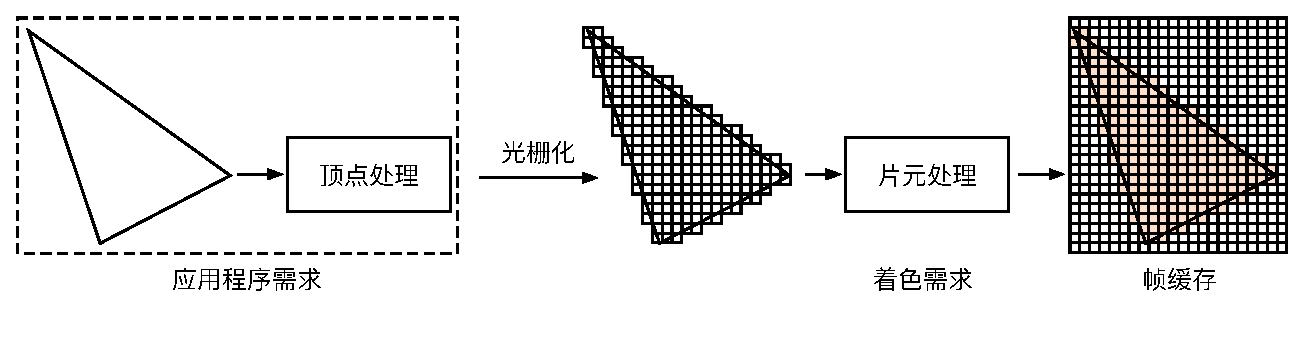
\includegraphics[width=\textwidth]{figures/api/vertex-pixel}
	\caption{OpenGL渲染管线的概念可以“简化”为顶点处理和片元处理,其中顶点处理着重于处理应用程序方面的需求,而片元处理着重于真正的着色计算。}
	\label{f:api-vertex-pixel}
\end{figure}



\subsection{顶点数据定义}
OpenGL渲染管线从宿主程序向OpenGL提交顶点及其他相关数据(如纹理,uniform/buffer块等),以及渲染管线可编程阶段使用的着色器程序开始,我们已经在前面的内容中讨论了其他一些数据对象,所以本节我们仅讨论顶点数据相关的定义。

顾名思义,顶点数组是一个数组数据,其数组的长度对应物体顶点的数量,每个数组元素表示的是一个或者多个顶点属性,顶点数组中的数据使用一个缓存对象来存储,称为顶点缓存对象(Vertex buffer object,VBO)\index{顶点缓存对象vertex buffer object}\index[en]{vertex buffer object顶点缓存对象}。由于每个顶点数据可能具有不同的数据类型及长度,所以同纹理一样,顶点属性也需要各种状态来告诉OpenGL在顶点着色器中应该怎样解析每个顶点的数据。

OpenGL使用一个顶点数组对象(Vertex Array Object,VAO)\index{顶点数组对象vertex array object}\index[en]{vertex array object顶点数组对象}来存储所有顶点数据相关的状态,例如每个顶点属性的格式,分量大小等状态信息,这和纹理,全局变量等其他数据的分散的状态管理是不一致,这是因为顶点数组相关的状态比较复杂,封装在一个容器对象中可以快速地在GPU内部进行状态切换,而不需要每次从客户内存重新上传众多的顶点状态数据。

顶点数组对象是一个普通的OpenGL对象,它使用glGenVertexArrays和glDeleteVertexArrays来创建和删除对象,并使用glBindVertexArray绑定顶点数组对象到当前上下文,以使后续的顶点数组相关的状态信息可以存储在该顶点数组对象中,但是顶点数组对象并没有绑定目标,因为顶点数组对象只能绑定到一种目标,所以OpenGL省略了这个绑定目标参数。当绑定一个当前的VAO对象之后,我们就可以开始设置各个顶点数据,这些顶点数据相关的状态会被自动捕捉到VAO对象之中。




\subsubsection{顶点属性}
在顶点着色器中,顶点属性变量使用in标识符定义,它的值由OpenGL根据相关设置从设备内存中读取到寄存器中,以下是顶点着色器中一些顶点属性的例子:

\begin{lstlisting}[language=C++]
in vec4 position;
in vec3 normal;
in vec2 texCoord[4];
\end{lstlisting}

每个顶点可以具有多个顶点属性变量,同纹理单元一样,OpenGL也使用一个整数索引来表示每个顶点属性,这个顶点属性索引值在着色器程序链接之后就可以通过以下命令直接获取:

\begin{lstlisting}[language=C++]
GLint glGetAttribLocation​(GLuint program​, const char *name​);
\end{lstlisting}

其中参数name即是顶点着色器中顶点属性变量的名称。同uniform/buffer块索引一样,顶点属性的索引值也可以直接在顶点着色器中定义,如:

\begin{lstlisting}[language=C++]
layout(location = 0) in vec4 vPosition;
\end{lstlisting}

当得到顶点属性的索引值之后,我们就可以设置每个顶点属性的值。默认情况下,每个顶点属性的值是一个常数,称为静态顶点属性,此时任何顶点着色器实例获得该顶点属性的值都是一样的,它相当于一个该顶点属性默认值,我们可以直接通过glVertexAttrib*相关的命令设置静态顶点属性的值\footnote{这种情况下的顶点属性数据也可以使用uniform变量代替。}。

静态顶点属性的值是直接存储在VAO中(而不是后面讲述的顶点缓存对象中)的,它为每个顶点属性分配一个具有4个分量的存储空间\footnote{这里的存储空间只是VAO专门用来存储静态顶点属性预留的一个4分量的数组空间,后面的顶点缓存对象并不遵循这样的约束。},其默认值为[0.0,0.0,0.0,1.0],因此一个标量顶点属性和一个vec4变量一样会占据一个完整的存储空间,所以通常我们倾向于尽可能将顶点数据合并进一个4分量矢量的大小,对于矩阵顶点属性,如$2\times 2$,$2\times 3$或$4\times 4$矩阵等,其每个列都会占据一个独立的存储空间。

但顶点属性更通常的使用方式是使用一个数组来对每个顶点存储不同的数据,OpenGL提供一个状态开关来开启顶点属性的数组形式,如图\ref{f:api-vertex-array}所示。​通过以下命令可以自两种状态之间切换:

\begin{lstlisting}[language=C++]
void glEnableVertexAttribArray(GLuint index​);
void glDisableVertexAttribArray(GLuint index​);
\end{lstlisting}

\begin{figure}
	\sidecaption
	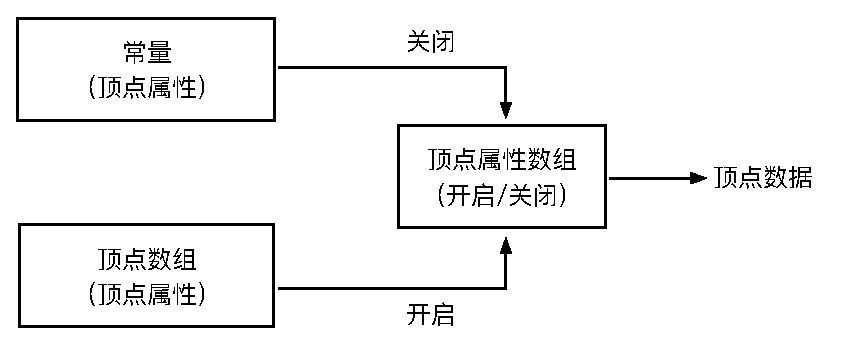
\includegraphics[width=0.65\textwidth]{figures/api/vertex}
	\caption{顶点属性变量的值默认是一个常量值,我们需要设置其是否使用数组的形式来对每个顶点分别存储不同的数据。}
	\label{f:api-vertex-array}
\end{figure}




\subsubsection{顶点缓存对象}
如果顶点属性数据使用数组的形式来存储,它的数据被存储于一个缓存对象中,称为顶点缓存对象(Vertex buffer object)\index{顶点缓存对象vertex buffer object}\index[en]{vertex buffer object顶点缓存对象},顶点缓存对象的绑定目标为GL\_ARRAY\_BUFFER。

当绑定一个顶点缓存对象之后,我们就可以将该顶点缓存对象绑定到某个顶点属性的索引值上,这通过以下命令来进行属性的绑定:

\begin{lstlisting}[language=C++]
void glVertexAttribPointer​(GLuint index​, GLint size​, GLenum type​, GLboolean normalized​, GLsizei stride​, const void *offset​);
void glVertexAttribIPointer​(GLuint index​, GLint size​, GLenum type​, GLsizei stride​, const void *offset​);
void glVertexAttribLPointer​(GLuint index​, GLint size​, GLenum type​, GLsizei stride​, const void *offset​);
\end{lstlisting}

这里offset即是绑定至目标为GL\_ARRAY\_BUFFER的缓存对象的偏移值,index表示顶点属性索引值,size表示的是每个顶点属性变量的尺寸,它表示的是其分量的数量(1,2,3,4),顶点缓存对象中每个分量的数据类型是由type决定的,type和size的可选值如表\ref{t:api-glVertexAttribPointer}所示。

\begin{table}
\begin{fullwidth}
\caption{设置顶点数组属性变量时指定的(每顶点)顶点数组尺寸及其每个顶点属性的数据类型,BGRA是一个特殊的标识符用来存储压缩数据类型(packed)。}
\label{t:api-glVertexAttribPointer}
\centering
\begin{tabular}{>{\small}p{0.3\thewidth}|>{\small}P{0.2\thewidth}|>{\small}p{0.17\thewidth}|>{\small}p{0.3\thewidth}}
\hline 
   命令名称 & sizes参数及其分量顺序 &整数处理 & 类型types参数  \\
    \hline  
  glVertexAttribPointer  &1,2,3,4,BGRA & 归一化或者非归一化的浮点数 &GLbyte, GLubyte, GLshort, GLushort, GLint, GLuint, GLfixed, GLfloat, GLhalf, GLdouble, packed\\
  glVertexAttribIPointer  &1,2,3,4     & 整数 & GLbyte, GLubyte, GLshort, GLushort, GLint, GLuint\\
  glVertexAttribLPointer  &1,2,3,4     & n/a & GLdouble\\


 \hline 
\end{tabular}
\end{fullwidth}
\end{table}

顶点缓存对象中的顶点数据以type参数对应的数据类型存储,type对应的每个分量所占存储的位数如表\ref{t:api-glVertexAttribPointer-type}所示,这些数据在被读进着色器的时候,会被不同的命令glVertexAttribPointer,glVertexAttribIPointer及glVertexAttribLPointer分别转化为三种对应的着色器中的数据类型:浮点型,整型及双精度浮点型,着色器数据类型和缓存中的数据类型并不是一一对应的,这些着色器中的数据类型和可匹配的顶点缓存数据类型的对应关系如表\ref{t:api-glVertexAttribPointer}所示,如果类型不匹配则会发生数据隐式转换。

\begin{myshaded}
顶点着色器中的顶点属性变量的类型只能是浮点型,整型或者双精度浮点型,实际上这和纹理数据在被读进着色器时进行的数据转换是类似的机制,GPU中通常只包含32位的寄存器,而不像CPU一样具有多种不同数据类型和大小的寄存器,所以GPU中更常使用的是32位的整数或32位的浮点数,其中对于有符号整数,它的其中一位用来存储符号,所以只有31位用来存储数据,对于双精度浮点数,它使用两个32位的寄存器来存储。由此可知,32位的浮点数只有很少的位数用来存储整数部分,如果整数部分取值范围比较大,最好直接使用整数存储或使用双精度的浮点数。
\end{myshaded}

对于glVertexAttribPointer命令,其顶点着色器中的数据类型为单精度浮点型,顶点缓存中的数据在被读进着色器的时候将根据normalized确定是否进行归一化。对于整数的归一化,它们分别被除以该数据类型可以包含的最大值\footnote{有符号整数要除去一位符号位。},根据type是否有无符号,而被转化到[0,1.0]和[-1.0,1.0]的范围,这和前面纹理数据读进着色器时的归一化是一样的方式;如果着色器中顶点属性变量类型和type的类型同时都是浮点数,则normalized始终为GL\_FLASE。此外,如果缓存对象中存储的是64位的双精度浮点型,则会被强制转化为32位的单精度浮点型。

glVertexAttribIPointer则不包含normalized参数,因为它直接将整数读进着色器,当然这也要求其缓存对象中的数据类型为整型,如表\ref{t:api-glVertexAttribPointer}所示;glVertexAttribLPointer也不包含normalized参数,因为归一化只发生在整型上,它有有限且固定的数据范围,浮点型本身进行归一化则没有太大意义。

stride参数用来表示数组中两个连续元素之间的字节偏移数,如果stride的值为0,则表示顶点缓存对象中的顶点属性是紧密排列的,所以OpenGL会根据分量的数量及数据类型来计算实际的偏移值,例如size为3,type为GL\_FLOAT,则OpenGL计算出的stride为12(每个浮点数占据4个字节,每个顶点属性变量具有3个分量 )。

stride和offset可以用来支持两种不同的定义顶点数组的方式,它们在C++中的数据结构类似如下:

\begin{lstlisting}[language=C++]
struct StructOfArrays
{
	GLfloat positions[VERTEX_COUNT * 3];
	GLfloat normals[VERTEX_COUNT * 3];
	GLubyte colors[VERTEX_COUNT * 4];
};
StructOfArrays structOfArrays;

struct Vertex
{
	GLfloat position[3];
	GLfloat normal[3];
	Glubyte color[4];
};

Vertex vertices[VERTEX_COUNT];
\end{lstlisting}

\begin{table}
\caption{glVertexAttriPoint()的数据类型标识符}
\label{t:api-glVertexAttribPointer-type}
\centering
\begin{tabular}{>{\small}p{0.48\textwidth}|>{\small}p{0.18\textwidth}|>{\small}p{0.31\textwidth}}
\hline 
   标识符 & OpenGL类型 & 位数  \\
    \hline  
  GL\_BYTE  							&GLbyte   & 有符号8位整型\\
  GL\_UNSIGNED\_BYTE  					&GLubyte  & 无符号8位整型\\
  GL\_SHORT  							&GLshort  & 有符号16位整型\\
  GL\_UNSIGNED\_SHORT  					&GLushort & 无符号16位整型\\
  GL\_INT  								&GLint    & 有符号32位整型\\
  GL\_UNSIGNED\_INT  					&GLuint   & 无符号32位整型\\
  GL\_FIXED  							&GLfixed  & 有符号16位定的型\\
  GL\_FLOAT                             &GLfloat  & 32位IEEE单精度浮点型\\
  GL\_HALF\_FLOAT                       &GLhalf   & 16位SIE5M10半精度浮点型\\
  GL\_DOUBLE                            &GLdouble & 64位IEEE双精度浮点型\\
  GL\_INT\_2\_10\_10\_10\_REV           &GLuint   & 32位压缩数据类型\\
  GL\_UNSIGNED\_INT\_2\_10\_10\_10\_REV &GLbyte   & 32位压缩数据类型\\


 \hline 
\end{tabular}
\end{table}


structOfArrays对象中每个顶点属性所有的数据分布构成一个数组,然后不同属性的数组存储在一个缓存对象中;而vertices数组中每个元素同时包含3个顶点属性;这样我们可以通过设置stride参数来精确告诉OpenGL该怎么获取每个顶点属性的数据。需要注意的是,这两种方式看起来是差不多的,但是它们之间的性能却是不一样的,后者能够充分利用第\ref{chp:hardware}章中学习的全局变量合并访问的机制,而前者导致每个相邻的顶点着色器实例读取的内存地址并不连续,所以性能较差。所以,在实践中,我们应该对每个顶点属性定义紧密排列的缓存对象。






\subsubsection{绘~~制}
定义好顶点数组后,OpenGL可以按照顶点数据中顶点元素的顺序进行渲染,然而这种由数组本身决定的顶点顺序并不灵活,例如一个人物会分为多个关节,各个关节之间会共享一些顶点数据,如果使用顶点数组本身的顺序来表示绘制时顶点的顺序,就会导致在渲染不同关节(或部分)的时候会出现重复的顶点数据,一个顶点可能包含多个顶点属性变量,因此这样的存储浪费极大;另一种情况是修改顶点的顺序则需要修改所有顶点属性对应的顶点缓存对象。

所以OpenGL使用单独的一个整型的数组来表示顶点的顺序,这称为索引数组,索引数组中元素的类型只能是UNSIGNED\_BYTE([0,255]), UNSIGNED\_SHORT([0,65535])或UNSIGNED\_INT([0,$2^{32}-1$]),宿主程序可以根据顶点的数量选择占用存储更少的整数类型。索引数组中的元素可以是重复的,这就是上述描述的顶点重复的部分,通过重复一个整型的索引值而不是重复多个顶点属性变量可以有效地减少存储空间的浪费。

OpenGL提供两种方式来定义顶点索引数组,一种是直接将客户内存中的顶点索引数组指针作为参数传递给绘制命令,另一种是将顶点索引数组存储在一个绑定到目标GL\_ELEMENT\_ARRAY\_BUFFER的缓存对象\footnote{顶点索引数组相关的绑定状态也被记录在VAO对象中。},这两种方式使用的绘制命令分别如下:

\begin{lstlisting}[language=C++]
void glDrawElements​(GLenum mode​, GLsizei count​, GLenum type​, void * indices​);
void glDrawArrays​(GLenum mode​, GLint first​, GLsizei count​);
\end{lstlisting}

以上两个命令也是OpenGL的两个基本的绘制命令,glDrawElements直接使用客户内存的顶点索引数据,并将其上传至设备内存,其type定义索引数组元素的类型,count定义顶点的数量;glDrawArrays使用顶点索引缓存对象中的索引数据,参数first表示缓存对象中顶点索引开始的偏移位置。

顶点索引数组仅仅是定义了顶点的顺序,这些信息还不足于判定其几何物体使用什么样的几何图元(Geometry primitive)\index{几何图元geometry primitive}\index[en]{geometry primitive几何图元}类型以及顶点索引中的哪些顶点构成一个基本的图元。物体基本几何图形的描述是至关重要的,例如几何着色器需要输入一个图元的数据,而光栅化器也需要根据图元来进行光栅化工作。

绘制命令中的mode参数就是用来定义图元类型的,它描述顶点索引数组中哪些索引值构成一个基础图元,以及图元的类型,mode的可选值包括:GL\_POINTS, GL\_LINE\_STRIP, GL\_LINE\_LOOP, GL\_LINES, GL\_LINE\_STRIP\_ADJACENCY, GL\_LINES\_ADJACENCY, GL\_TRIANGLE\_STRIP, GL\_TRIANGLE\_FAN, GL\_TRIANGLES, GL\_TRIANGLE\_STRIP\_ADJACENCY, GL\_TRIANGLES\_ADJACENCY以及 GL\_PATCHES,其中*\_ADJACENCY相关的图元类型是专用于给几何着色器提供信息的,这部分内存将在后面讲述,部分图元类型参见图\ref{f:api-primitives}所示。

\begin{figure}
	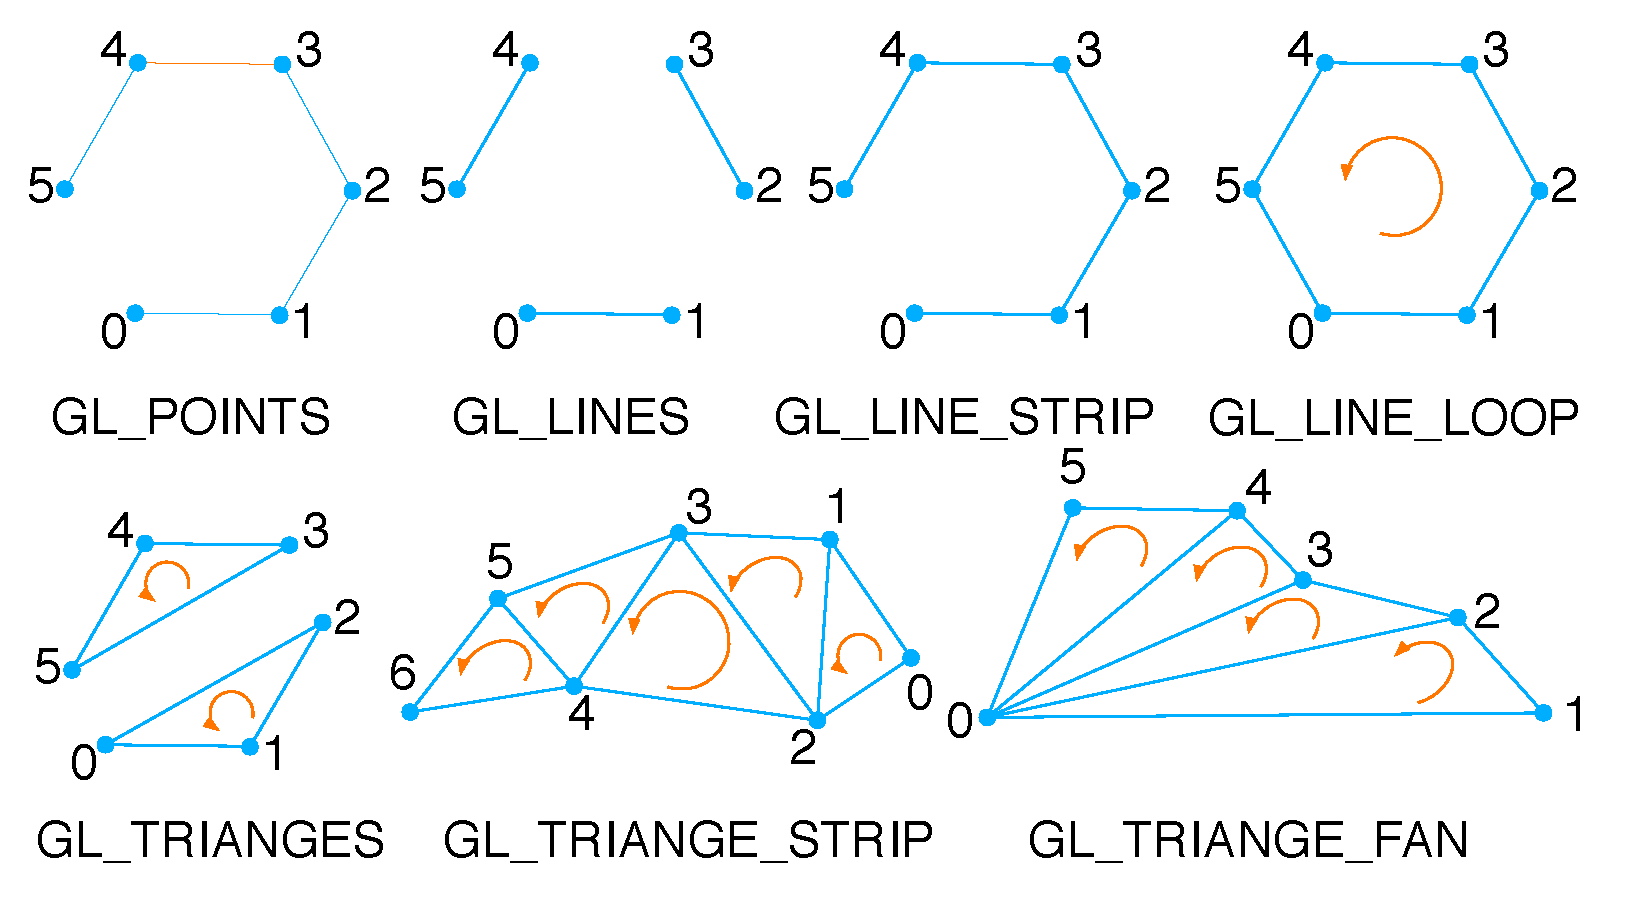
\includegraphics[width=\textwidth]{figures/api/primitives}
	\caption{部分OpenGL图元类型,图元类型定义了顶点索引数组中哪些索引值用来构成一个基础图元,以及基础图元的类型。}
	\label{f:api-primitives}
\end{figure}





\paragraph{多次合并绘制}
分析图\ref{f:api-primitives}中的下面的三个图元类型,其中GL\_TRIANGE\_STRIP和GL\_TRIANGE\_FAN类型充分利用图元的相邻性来重用顶点(这也是使用顶点索引数组的好处),而GL\_TRIANGES则对每个图元都完整定义每个顶点,其顶点重复率很高,在这种类型中,顶点索引数组中顶点的顺序和顶点数组本身的顺序是一致的。

这种利用之前的共享顶点来构成新图元的方式虽然节省了存储空间,但也带来了一个新的问题:即这些图元必须是相邻的。如果有多个物体使用完全一样的着色器及图元类型,但是它们分别属于不同的物体,这却不得不分别调用多次绘制命令,因为共享顶点的图元类型没法将它们从几何空间上分开(非共享的GL\_TRIANGES虽然可以任意从空间分开各个图元,但又造成极大的存储空间浪费),而一次新的绘制导致的VAO的绑定和修改的成本都是极高的。

为了优化这种多次相似的绘制(使用相同的着色器及图元类型),例如场景中存在大量相同类型的物体分布在空间中不同的地方,这些物体可以使用以下命令进行一次性绘制:

\begin{lstlisting}[language=C++]
void glMultiDrawArrays​( GLenum mode​, GLint *first​, GLsizei *count​, GLsizei primcount​);
\end{lstlisting}

这在功能上类似于:

\begin{lstlisting}
void glMultiDrawArrays( GLenum mode, GLint *first, GLsizei *count, GLsizei primcount )
{
	for (int i = 0; i < primcount; i++)
	{
		if (count[i] > 0)
			glDrawArrays(mode, first[i], count[i]);
	}
}
\end{lstlisting}

即对每个物体分别调用一次绘制以使每个物体的图元在空间上的位置分开,但是在内部OpenGL会使用一次绘制命令\footnote{其实这很简单,OpenGL只需要在向几何着色器提供每个图元的顶点集合的时候能够正确地找到对应的图元的顶点即可,例如它可以像后面的图元重启那样记录一些“断点”,在遇到这些点的时候重新从下一个顶点开始新的图元绘制即可。}。需要注意的是,使用多次合并绘制的所有顶点数据必须来源于同一个VAO对象中,每个分离的几何物体在顶点索引数组中的起始位置分别通过first和count数组来定义,primcount则表示几何物体的数量。

该机制对应glDrawElements的版本则是:

\begin{lstlisting}[language=C++]
void glMultiDrawElements​( GLenum mode​, GLsizei *count​, GLenum type​, void **indices​, GLsizei primcount​ );
\end{lstlisting}

利用图元重启的机制也可以实现类似的功能,该机制向OpenGL提供一个索引值,如果该索引值在顶点索引数组中被找到,则OpenGL将该索引顶点抛弃,并且从该顶点的下一个索引顶点开始重新计算新的图像,如图\ref{f:api-primitive-restart}所示。但是该机制只能处理两个空间上分离的物体。

\begin{figure}
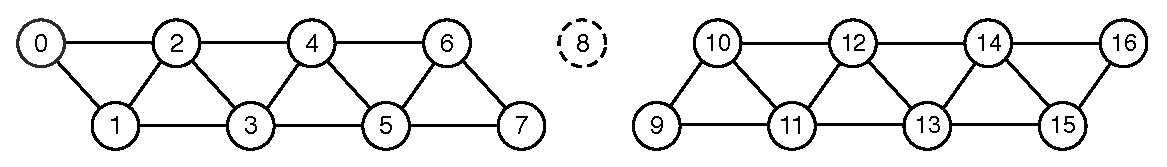
\includegraphics[width=\textwidth]{figures/api/primitive-restart}
	\caption{使用图元重启动的特性打断三角形条带}
	\label{f:api-primitive-restart}
\end{figure}

使用图元重启需要开启GL\_PRIMITIVE\_RESTART设置,它和对应的设置命令如下:

\begin{lstlisting}[language=C++]
glEnable(GL_PRIMITIVE_RESTART)​;
void glPrimitiveRestartIndex(GLuint index​);
\end{lstlisting}





\paragraph{多实例绘制}
多次合并绘制适合多个独立物体“相似”的绘制,每个物体拥有独立的顶点数据用来保证每个物体被正确绘制。假设现有多个完全相同的物体,它们拥有完全一样的顶点属性数据,只是具有少量不同的部分(例如不同的位置属性),如果我们使用多次合并绘制则需要分别在一个顶点缓存对象中存储各自对应的顶点数据(这些几乎完全是重复的),虽然我们可以对每次绘制设置相同的顶点数组的位置来使用同一套顶点数据,但是那样我们几乎完全无法在着色器中区分不同的实例,因此无法对其不同的部分作出相应的修改。

多实例绘制(Instanced rendering)\index{多实例绘制instanced rendering}\index[en]{instanced rendering多实例绘制}对完全相同的顶点数据绘制多次,但是它在着色器内提供一个几何体实例变量gl\_InstanceID来使着色器可以决定对不同的实例进行适当的修改(例如读取uniform/buffer块数据中的某个表数据),多实例绘制使用以下命令对同一套顶点属性数据绘制多次:

\begin{lstlisting}
void glDrawArraysInstanced​(GLenum mode​, GLint first​, GLsizei count​, GLsizei instancecount​);
void glDrawElementsInstanced​(GLenum mode​, GLsizei count​, GLenum type​, const void *indices​, GLsizei instancecount​);
\end{lstlisting}

其中,instancecount表示几何体实例的数量,对于每个实例,内置变量gl\_InstanceID都会一次递增,新的数值会被传递到着色器,以区分不同实例的顶点属性,其他参数则和基本的绘制类型一样。

多实例绘制特性需要通过以下命令来启用:

\begin{lstlisting}[language=C++]
void VertexAttribDivisor( uint index, uint divisor );
\end{lstlisting}

这里index表示顶点属性索引值,divisor表示当前属性的更新频率值,如果divisor为0(这也是其默认值), 则多实例绘制将被禁止,几何体按照正常的方式绘制,每个顶点都会被分配到一个独立的属性值;如果divisor是一个非0值,那么该顶点属性将启用多实例特性,此时OpenGL从属性数组中每隔divisor个实例都会读取一个新的数值(而不是之前的每个顶点)。此时在这个属性对应的顶点属性数组中,数据索引值的计算变成instance/divisor的形式,其中instance表示当前的实例数目。如果divisor值为1,它表示在顶点着色器中每个实例中的所有顶点都会共享同一个属性值,如果divisor为2,那么每两个实例会共享同一个属性值,以此类推。利用此机制,我们可以实现比如传递给每个几何体一个不同的模型视图变换矩阵等。





\paragraph{间接绘制}
此外,OpenGL还支间接绘制(Indirect rendering)\index{间接绘制indirect rendering}\index[en]{indirect rendering间接绘制},它的大部分绘制参数(例如顶点开始位置以及顶点的数量等)来自于一个绑定到GL\_DRAW\_INDIRECT\_BUFFER绑定目标的缓存对象。

间接绘制的目的是避免不必要的GPU->CPU->GPU的数据复制操作,在OpenGL中,有时候顶点数据来自于渲染管线的中间产物(如变换反馈缓存),甚至直接由计算着色器或其他GPU计算产生的计算结果,这个时候这些缓存对象中的顶点的顺序,以及绘制相关的一些参数也是有GPU直接设置的,如果使用传统的绘制命令,则需要将这些参数都读回到CPU,然后再以参数的方式复制到GPU,造成一些不必要的开支。因此间接绘制命令直接可以从一个缓存对象中读取绘制命令需要的参数。

间接绘制机制支持全部普通的OpenGL绘制命令,例如多次合并绘制,多实例绘制等,它们对应的绘制命令名称分别为原始绘制命令名称后面加上Indirect,例如:

\begin{lstlisting}
void glDrawArraysIndirect​(GLenum mode​, const void *indirect​);
\end{lstlisting}

根据顶点索引数据存储是否存储在缓存对象中,间接绘制参数缓存对象中的数据具有不同的数据结构,对于索引数据由客户内存直接提供的(如上述的glDrawArraysIndirect),它的数据结构如下:

\begin{lstlisting}
typedef  struct 
{
   	GLuint  count;
   	GLuint  instanceCount;
   	GLuint  first;
   	GLuint  baseInstance;
} DrawArraysIndirectCommand;
\end{lstlisting}

对于有顶点索引缓存提供的索引数组,对于的数据结构则为:

\begin{lstlisting}
typedef  struct 
{
    GLuint  count;
    GLuint  instanceCount;
    GLuint  firstIndex;
    GLuint  baseVertex;
    GLuint  baseInstance;
} DrawElementsIndirectCommand;
\end{lstlisting}


\begin{comment}
	


\subsection{顶点着色器}
投射,变换,摄像机
\subsection{细分着色器}
\subsection{几何着色器}
多层渲染
\section{片元处理}
\subsection{片元着色器}
https://www.opengl.org/wiki/Fragmentz

\subsection{每片元操作}
\section{计算着色器}





\end{comment}































